\documentclass[11pt,a4paper]{article}

% -----------------------------------------------------------------------------
% PACKAGES & CONFIGURATION
% -----------------------------------------------------------------------------
\usepackage[utf8]{inputenc}
\usepackage[T1]{fontenc}
\usepackage{lmodern}
\usepackage{microtype}
\usepackage[margin=1.8cm,top=2.0cm,bottom=2.0cm,headheight=14pt]{geometry}
\usepackage{graphicx}
\usepackage{xcolor}
\usepackage{fancyhdr}
\usepackage{titlesec}
\usepackage{amsmath,amssymb}
\usepackage{booktabs}
\usepackage{array}
\usepackage{caption}
\usepackage{float}
\usepackage{subcaption}
\usepackage{needspace}
\usepackage{tcolorbox}
\tcbuselibrary{skins,listings}
\usepackage{hyperref}

% -----------------------------------------------------------------------------
% COLOR DEFINITIONS (ENSIA Lab Theme)
% -----------------------------------------------------------------------------
\definecolor{primary}{RGB}{31, 78, 121}        % Deep Navy Blue (#1f4e79)
\definecolor{darktext}{RGB}{30, 30, 30}        % Text color
\definecolor{codebg}{RGB}{246, 247, 249}       % Shaded code box background
\definecolor{codeborder}{RGB}{195, 205, 215}   % Code box border
\definecolor{barcolor}{RGB}{31, 78, 121}       % Left accent bar

% -----------------------------------------------------------------------------
% GRAPHICS PATH
% -----------------------------------------------------------------------------
\graphicspath{{screenshots/}}

% -----------------------------------------------------------------------------
% HEADERS & FOOTERS (Matching ENSIA Lab Sheet)
% -----------------------------------------------------------------------------
\pagestyle{fancy}
\fancyhf{}
\fancyhead[L]{\small\textit{ENSIA -- AI and Data Science}}
\fancyhead[R]{\small\textit{Introduction to Mobile Robotics}}
\fancyfoot[L]{\small\textit{Lab 2: CoppeliaSim \& Differential Drive Modeling -- Solution Report}}
\fancyfoot[R]{\small\textit{Page \thepage}}
\renewcommand{\headrulewidth}{0.5pt}
\renewcommand{\footrulewidth}{0.5pt}

% -----------------------------------------------------------------------------
% SECTION TITLE FORMATTING
% -----------------------------------------------------------------------------
\titleformat{\section}
  {\color{primary}\Large\bfseries}{\thesection.}{0.6em}{}

\titleformat{\subsection}
  {\color{primary}\large\bfseries}{}{0pt}{}

\titleformat{\subsubsection}
  {\color{primary}\normalsize\bfseries}{}{0pt}{}

\titlespacing*{\section}{0pt}{10pt plus 1pt minus 1pt}{5pt}
\titlespacing*{\subsection}{0pt}{8pt plus 1pt minus 1pt}{4pt}
\titlespacing*{\subsubsection}{0pt}{6pt plus 1pt minus 1pt}{3pt}

% -----------------------------------------------------------------------------
% COMMAND BOX STYLING
% -----------------------------------------------------------------------------
\newtcblisting{cmdbox}{
  enhanced,
  colback=codebg,
  colframe=barcolor,
  arc=1.0mm,
  leftrule=2.5pt,
  rightrule=0.4pt,
  toprule=0.4pt,
  bottomrule=0.4pt,
  boxsep=0.2mm,
  left=2.5mm,
  right=2.5mm,
  top=1.0mm,
  bottom=1.0mm,
  listing only,
  listing options={
    basicstyle=\footnotesize\ttfamily,
    breaklines=true,
    columns=fullflexible,
    keepspaces=true,
    showstringspaces=false
  }
}

\captionsetup{
  font=small,
  labelfont={bf,color=primary},
  labelsep=period,
  skip=4pt
}

\hypersetup{
  colorlinks=true,
  linkcolor=primary,
  citecolor=primary,
  urlcolor=primary,
  pdfauthor={BELHIMER Mohamed Ayoub},
  pdftitle={LAB 2 REPORT - BELHIMER Mohamed Ayoub - Group 1}
}

% -----------------------------------------------------------------------------
% DOCUMENT BODY
% -----------------------------------------------------------------------------
\begin{document}

% -----------------------------------------------------------------------------
% DIRECT SOLUTION HEADER
% -----------------------------------------------------------------------------
\begin{center}
  {\LARGE \textbf{\color{primary}LAB 2 REPORT}}\\[0.25cm]
  {\large \textbf{BELHIMER Mohamed Ayoub} \quad \textbullet \quad \textbf{Group 1}}\\[0.25cm]
  \rule{\linewidth}{0.8pt}
\end{center}
\vspace{-0.1cm}

% =============================================================================
% SECTION 1: COPPELIASIM SIMULATOR
% =============================================================================
\section{CoppeliaSim Simulator}
\subsection*{1.3 Tasks}

\subsubsection*{Task 1: CoppeliaSim Simulator Overview}
According to the CoppeliaSim manual, the simulator provides:
\begin{itemize}
  \item \textbf{Distributed Architecture:} Control robots via Lua/Python scripts, ROS/ROS 2 nodes, or Remote APIs (C++, Python).
  \item \textbf{Physics Engines:} Built-in support for Bullet, ODE, MuJoCo, and Vortex dynamics.
  \item \textbf{Sensors \& Actuators:} Built-in proximity sensors, 2D/3D LiDARs, vision sensors, and encoders.
  \item \textbf{Modular Models:} Portable \texttt{.ttm} model files containing geometry, physics, and scripts.
\end{itemize}

% =============================================================================
% TASK 2: SENSOR EXPLORATION AND CLASSIFICATION
% =============================================================================
\subsubsection*{Task 2: Sensor Exploration and Classification}
The Model Browser under \texttt{components/sensors} contains various robotic sensors:

\begin{figure}[H]
  \centering
  \begin{subfigure}[b]{0.48\linewidth}
    \centering
    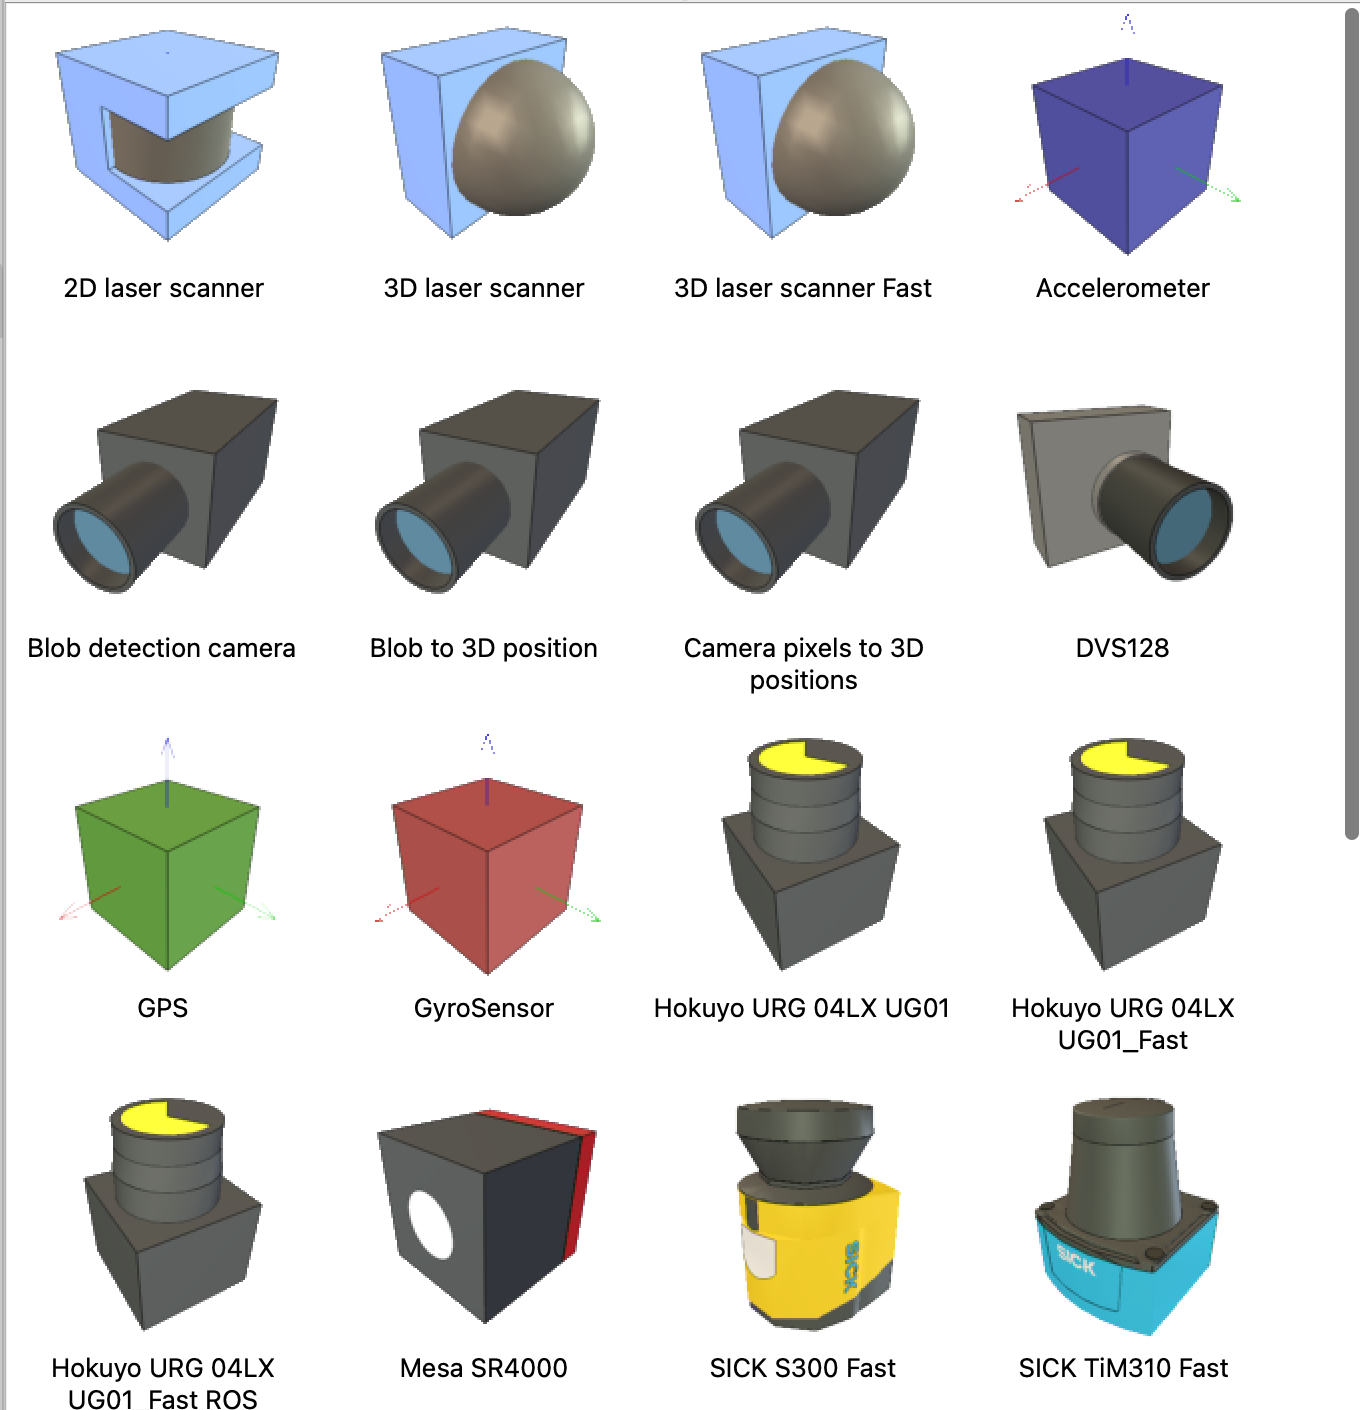
\includegraphics[width=\linewidth]{fig_task2_sensors_1.png}
  \end{subfigure}
  \hfill
  \begin{subfigure}[b]{0.48\linewidth}
    \centering
    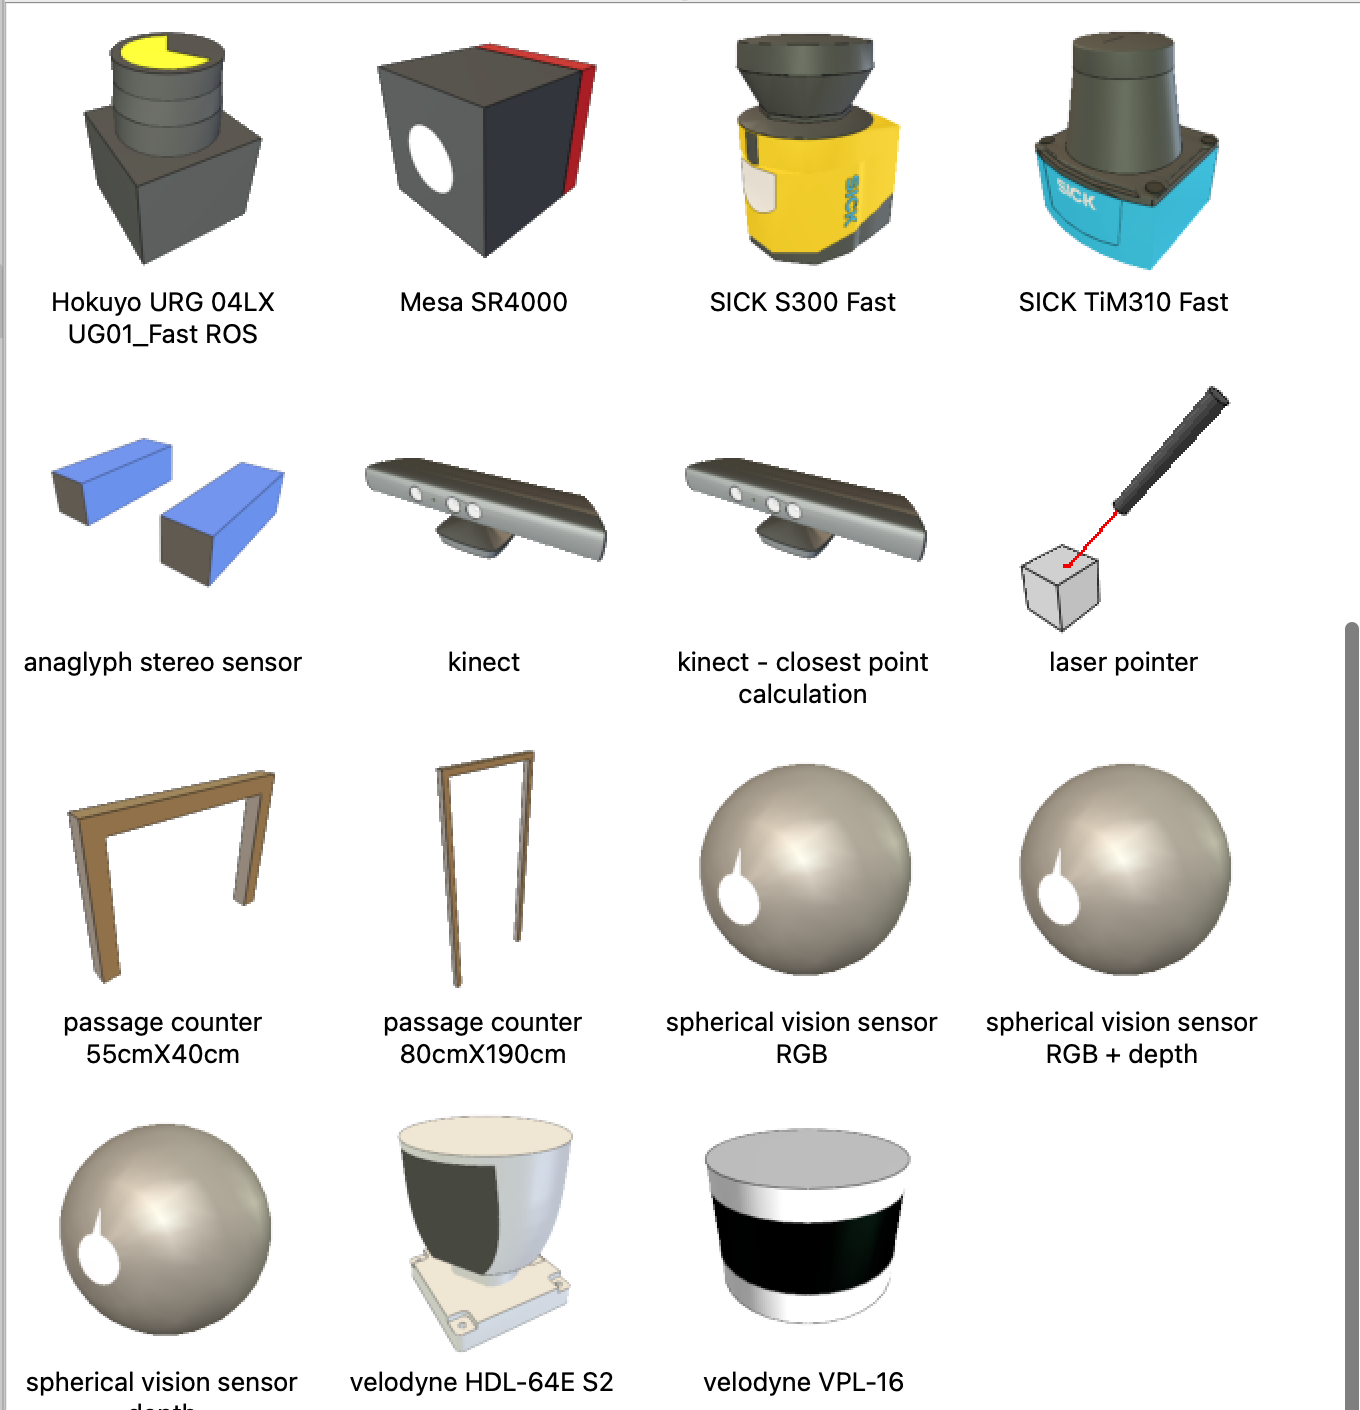
\includegraphics[width=\linewidth]{fig_task2_sensors_2.png}
  \end{subfigure}
  \caption{CoppeliaSim Model Browser displaying available sensor models under \texttt{components/sensors}.}
  \label{fig:sensors_browser}
\end{figure}

\paragraph{(a) Three Identified Sensor Types:}
\begin{enumerate}
  \item \textbf{2D Laser Scanner (LiDAR)} (e.g., \textit{Hokuyo URG 04LX UG01})
  \item \textbf{RGB-D Vision Sensor} (e.g., \textit{Kinect})
  \item \textbf{Inertial Sensor (IMU)} (e.g., \textit{Accelerometer} / \textit{GyroSensor})
\end{enumerate}

\paragraph{(b) Functional Description:}
\begin{itemize}
  \item \textbf{2D Laser Scanner (LiDAR):} Measures distances to surrounding surfaces using Time-of-Flight (ToF) laser pulses across a 2D plane. It is used for obstacle avoidance, 2D SLAM, and building occupancy grid maps.
  \item \textbf{RGB-D Sensor (Kinect):} Combines an RGB camera with an infrared depth sensor to output color images and 3D point clouds. It is used for 3D environment mapping and visual object recognition.
  \item \textbf{Inertial Measurement Unit (IMU):} Measures linear acceleration with an accelerometer and angular velocity with a gyroscope. It provides high-frequency motion tracking and assists in robot state estimation.
\end{itemize}

\paragraph{(c) Proprioceptive vs. Exteroceptive Sensors:}
\begin{itemize}
  \item \textbf{Proprioceptive sensors:} Measure internal states of the robot (e.g., wheel encoders, motor current, battery level, accelerometers, gyroscopes).
  \item \textbf{Exteroceptive sensors:} Measure signals from the external environment (e.g., LiDAR, sonar, cameras, bump sensors, GPS).
\end{itemize}

% =============================================================================
% TASK 3: WHEELED MOBILE ROBOT MODELS
% =============================================================================
\subsubsection*{Task 3: Wheeled Mobile Robot Exploration}
The Model Browser under \texttt{robots/mobile} contains various mobile robotic platforms:

\begin{figure}[H]
  \centering
  \begin{subfigure}[b]{0.48\linewidth}
    \centering
    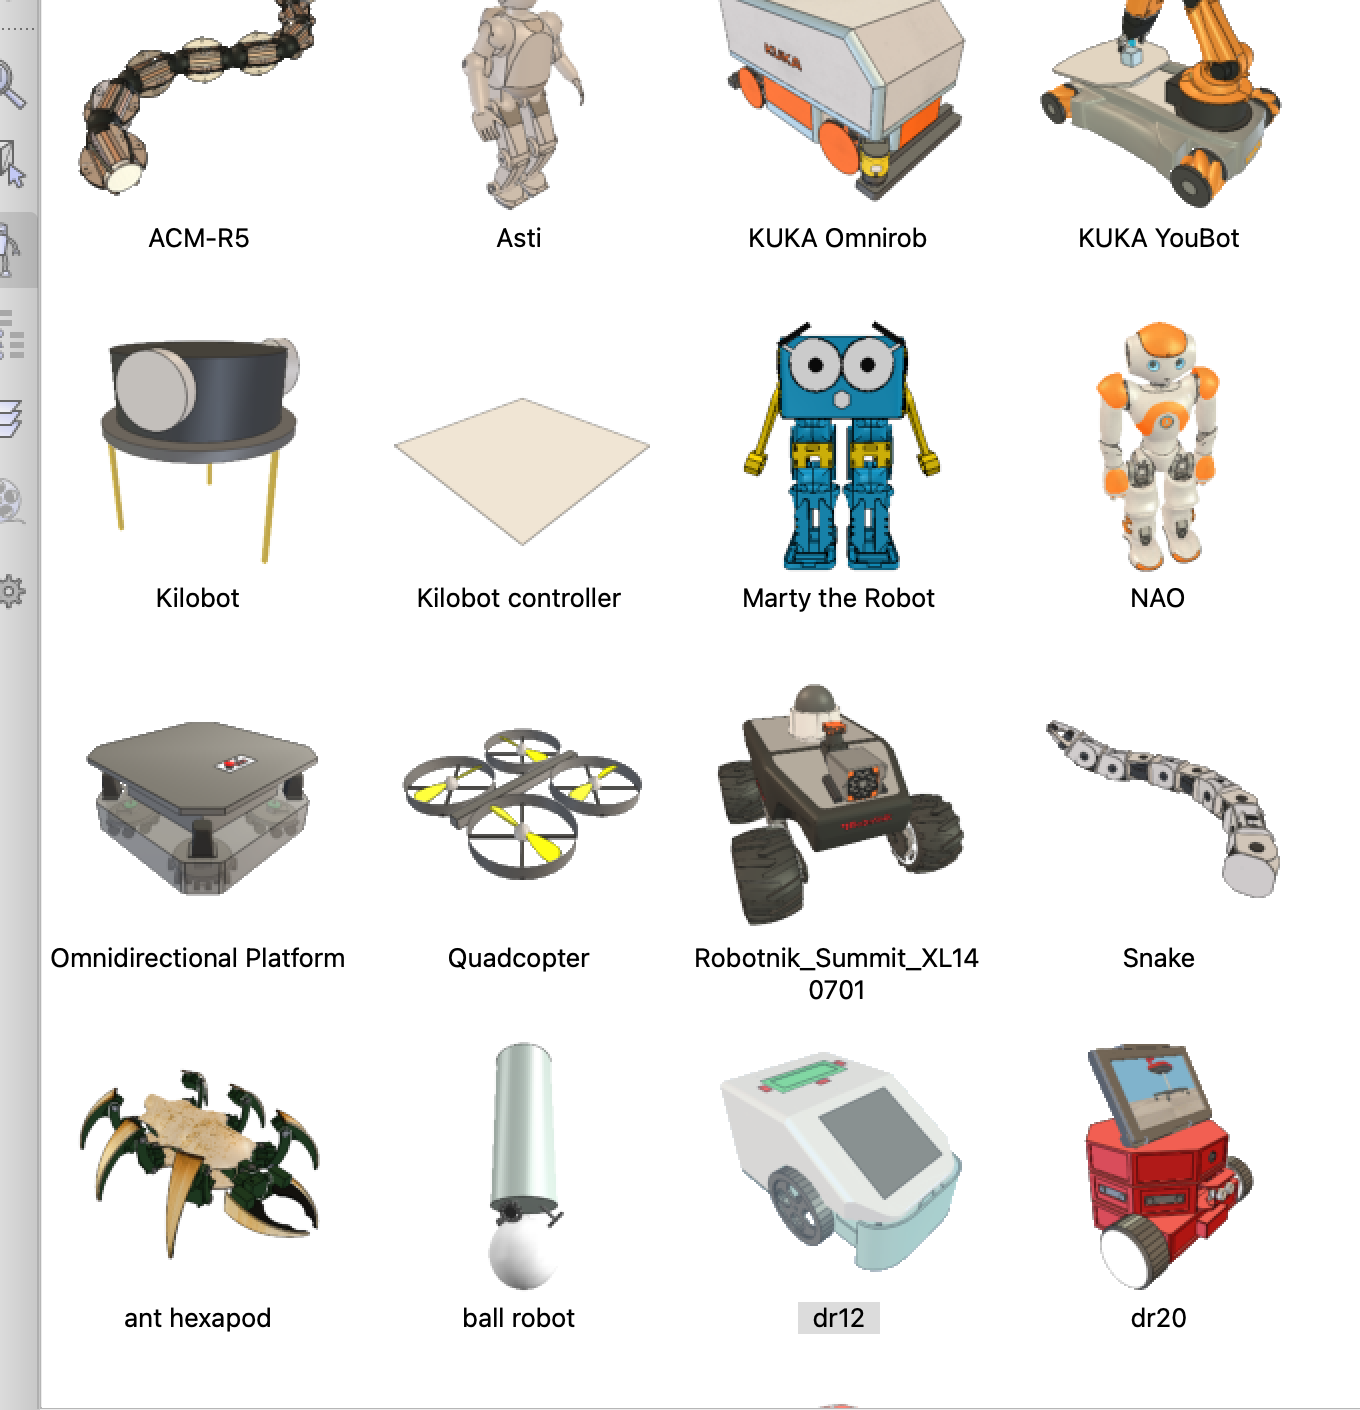
\includegraphics[width=\linewidth]{fig_task3_robots_1.png}
  \end{subfigure}
  \hfill
  \begin{subfigure}[b]{0.48\linewidth}
    \centering
    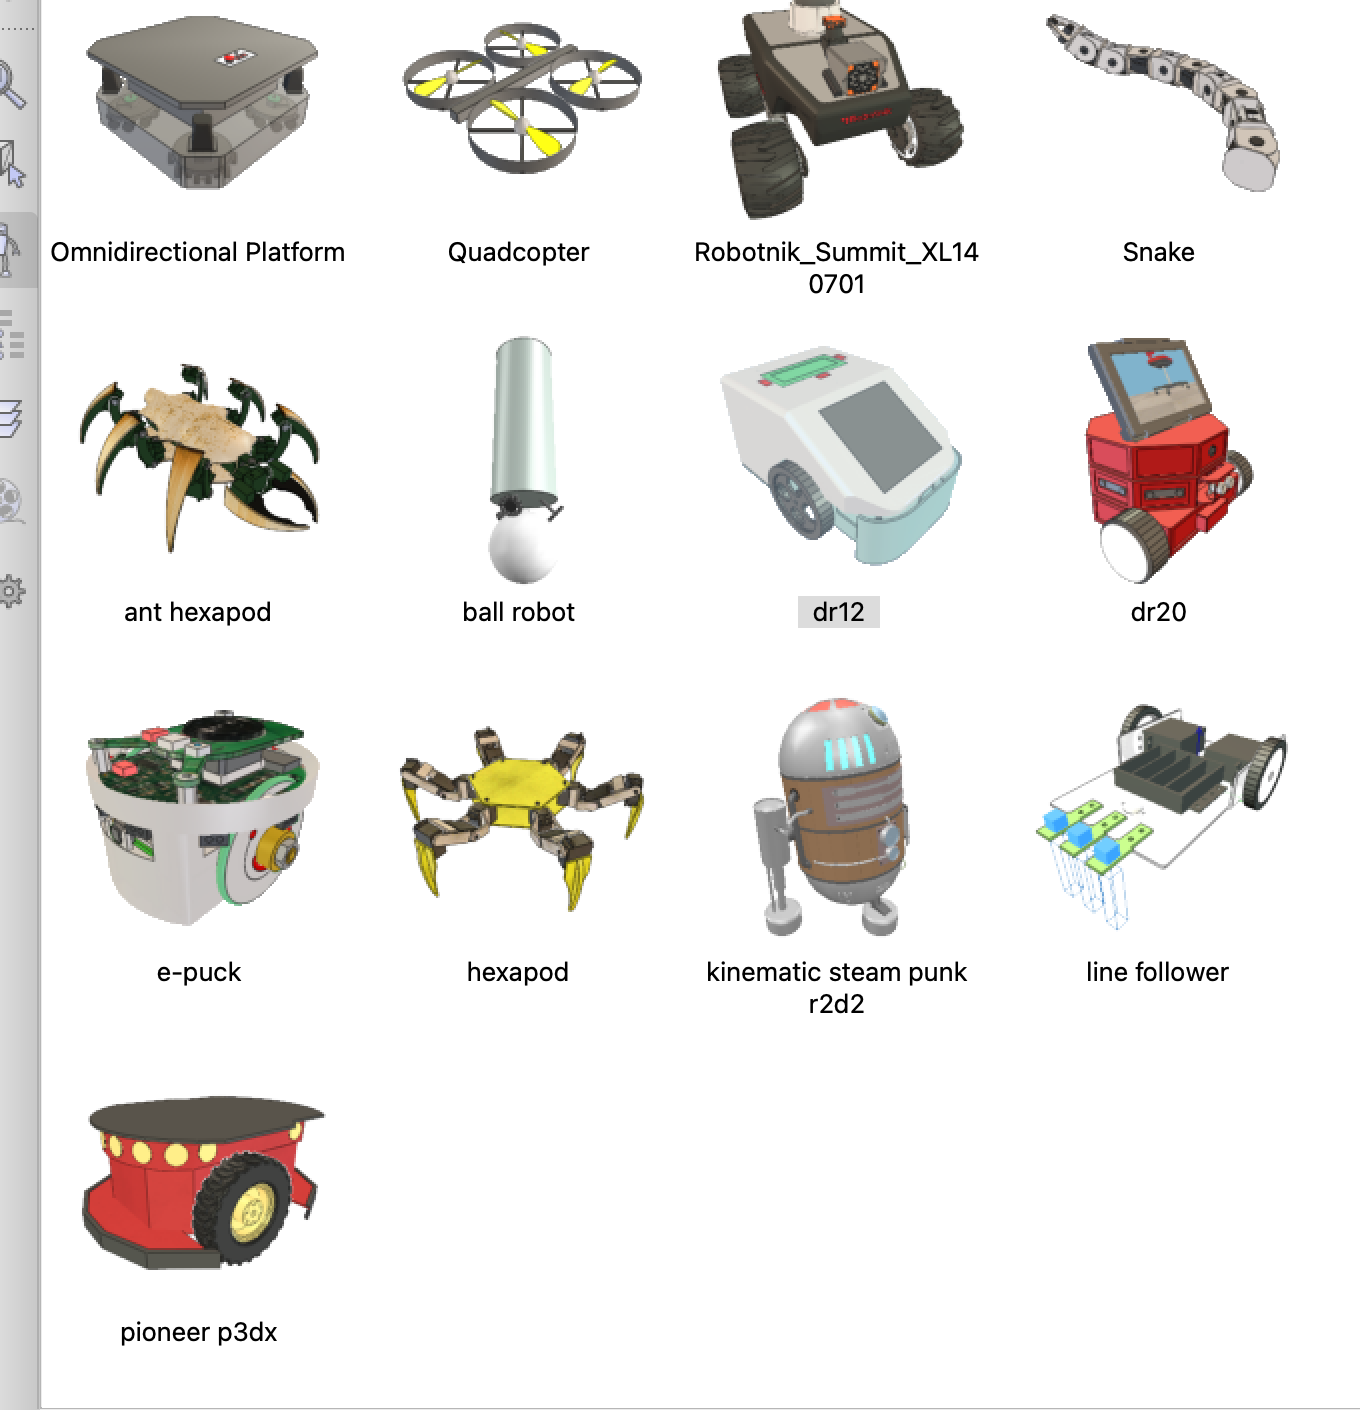
\includegraphics[width=\linewidth]{fig_task3_robots_2.png}
  \end{subfigure}
  \caption{CoppeliaSim Model Browser displaying available mobile robots under \texttt{robots/mobile}.}
  \label{fig:robots_browser}
\end{figure}

\paragraph{(a) \& (b) Identified Mobile Robot Types:}
\begin{enumerate}
  \item \textbf{Pioneer P3DX} (Differential Drive)
  \item \textbf{KUKA YouBot} (Omnidirectional Drive)
  \item \textbf{Robotnik Summit XL} (4WD Differential Drive)
\end{enumerate}

\paragraph{(c) Wheel Configuration Description:}
\begin{itemize}
  \item \textbf{Pioneer P3DX (Differential Drive):} Two independently driven coaxial wheels on a central axis, with a rear passive caster for balance. Straight motion uses equal wheel velocities; turning uses a differential velocity between left and right wheels.
  \item \textbf{KUKA YouBot (Omnidirectional Drive):} Four Mecanum wheels (also known as Swedish wheels) with $45^\circ$ passive rollers. Allows holonomic 3-DOF planar motion (instant translation in $x, y$ and rotation $\theta$ without needing to turn its body first).
  \item \textbf{Robotnik Summit XL (4WD Differential Drive):} Four fixed-axis driven wheels (two per side). Turning is achieved identically to tracked tanks: the left-side and right-side wheels are driven at different speeds, forcing the tires to intentionally slip (skid) laterally across the ground to reorient.
\end{itemize}

% =============================================================================
% TASK 4: ROBOT INSTANTIATION & SIMULATION
% =============================================================================
\subsubsection*{Task 4: Robot Instantiation and Simulation Run}
Robot models were dragged from the Model Browser into the scene and the simulation was started.

\begin{figure}[H]
  \centering
  \begin{subfigure}[b]{0.48\linewidth}
    \centering
    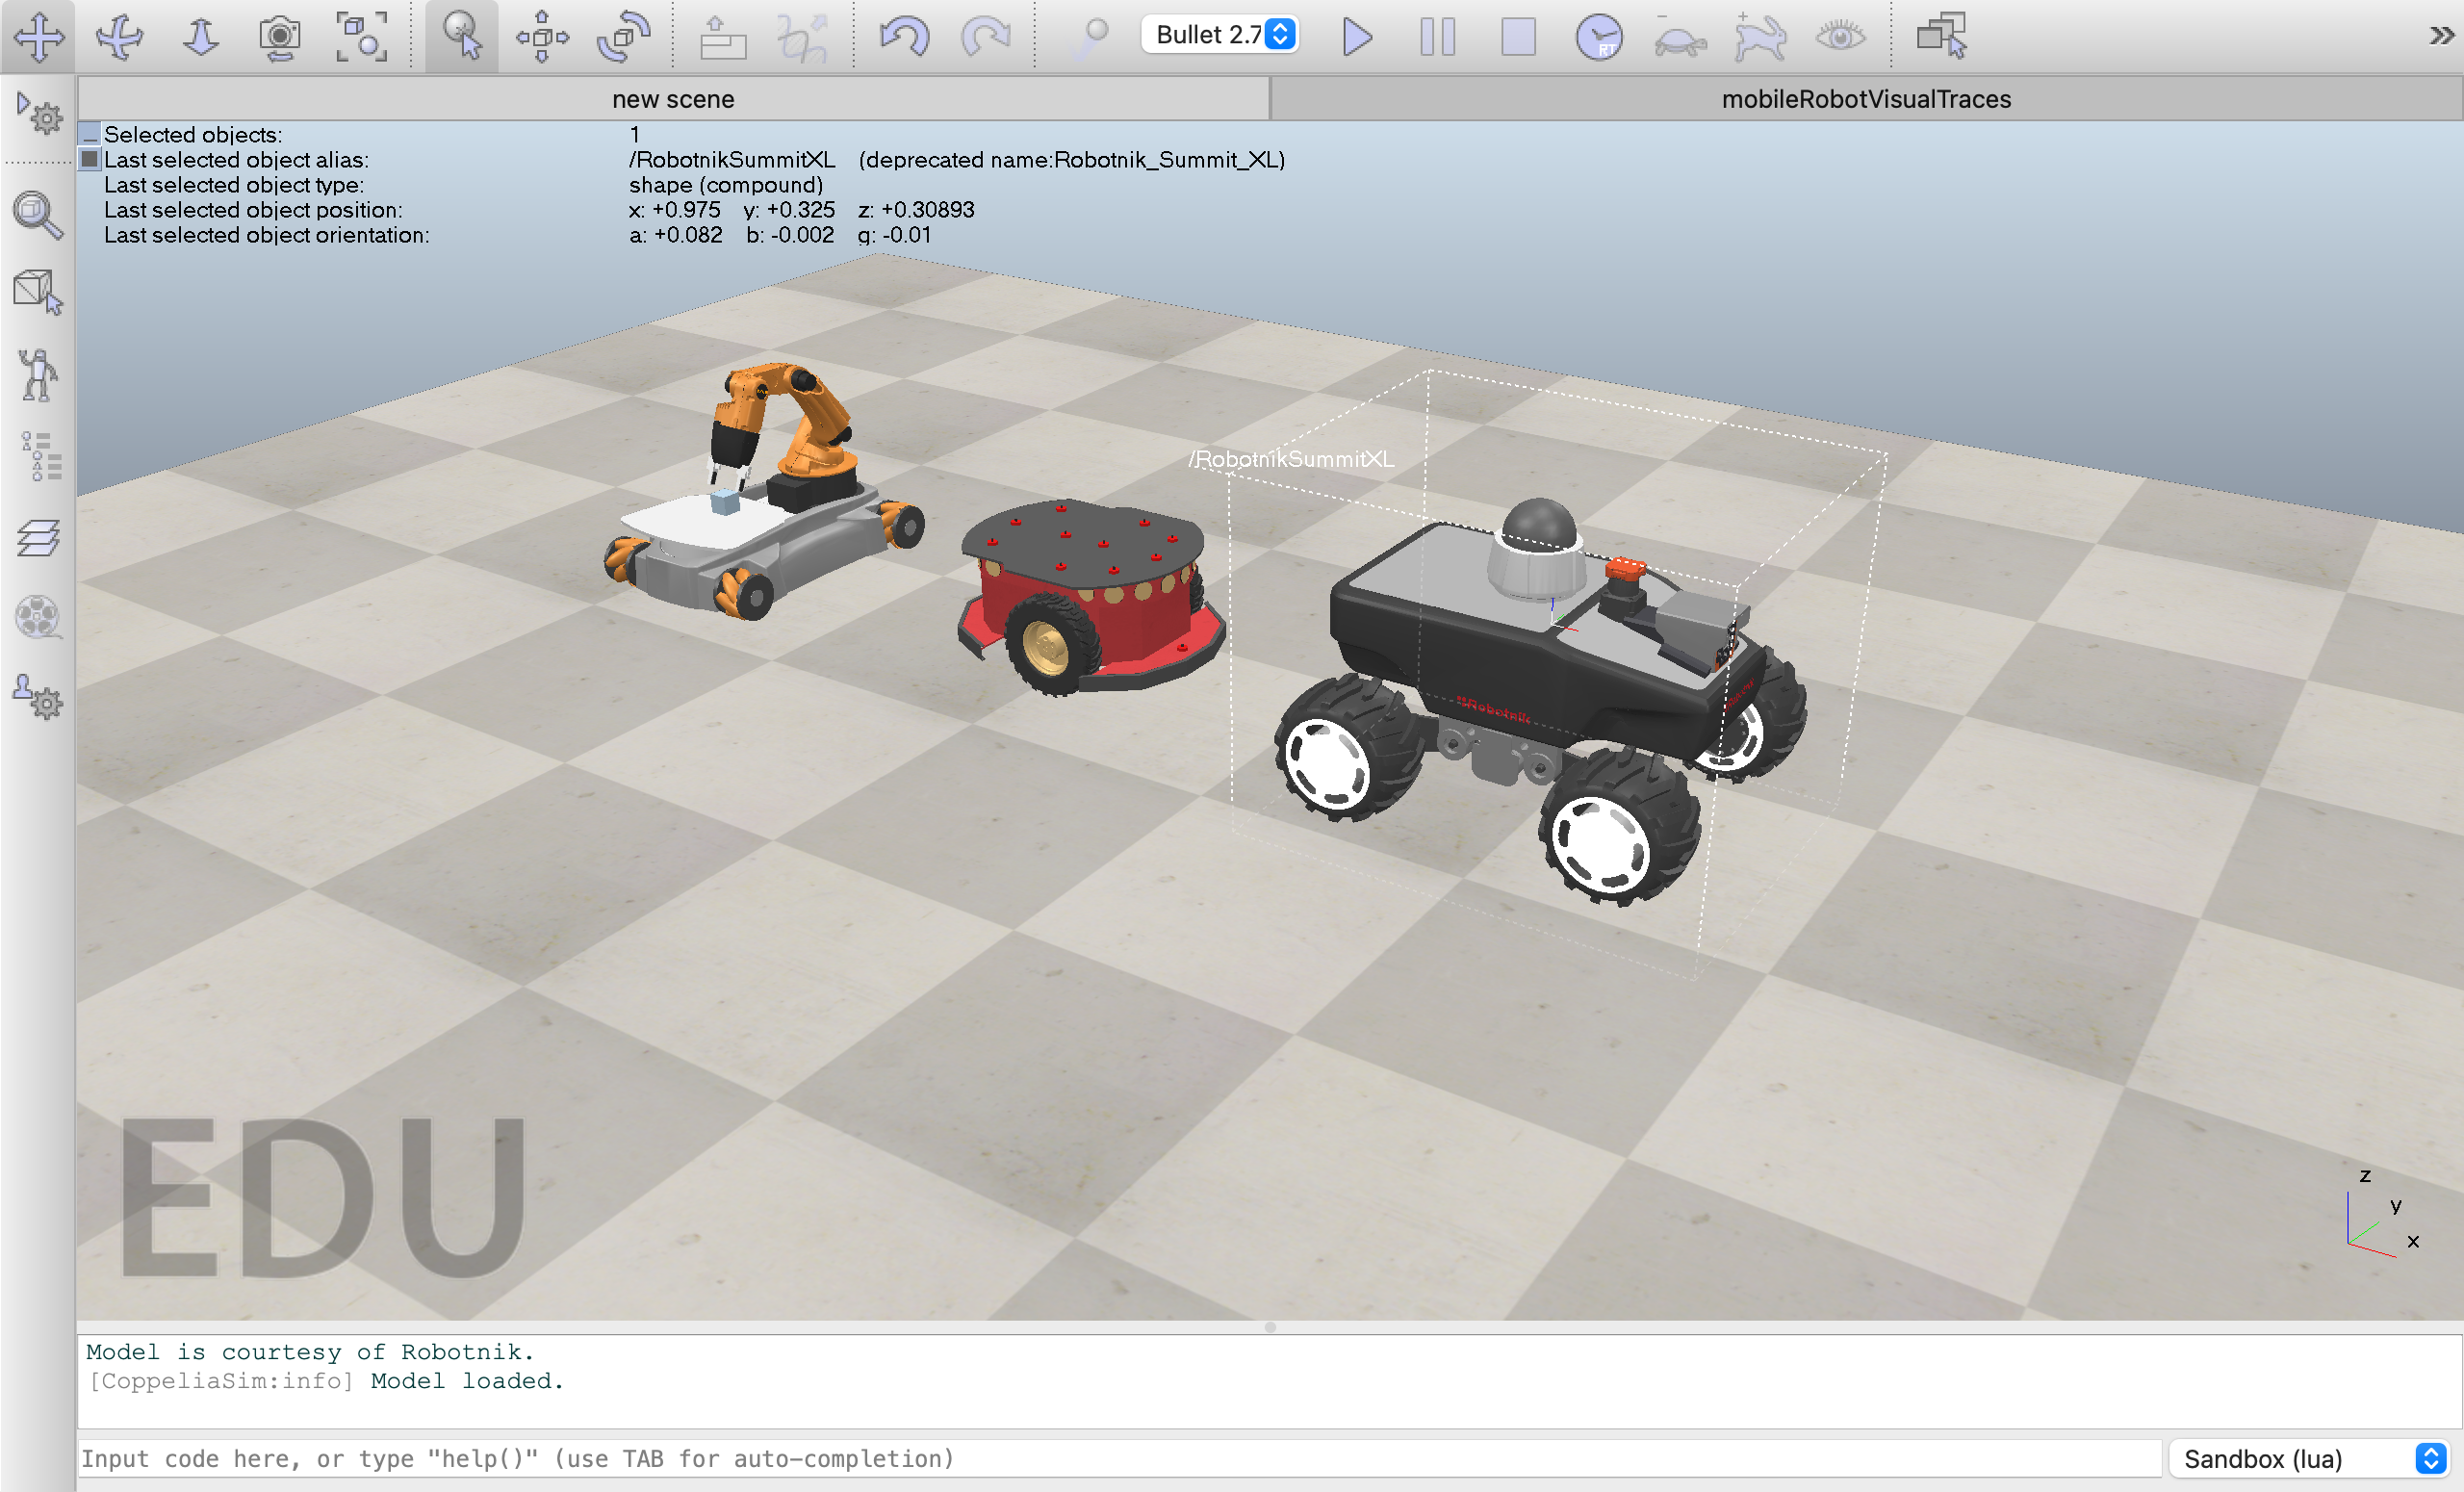
\includegraphics[width=\linewidth]{fig_task4_simulation.png}
  \end{subfigure}
  \hfill
  \begin{subfigure}[b]{0.48\linewidth}
    \centering
    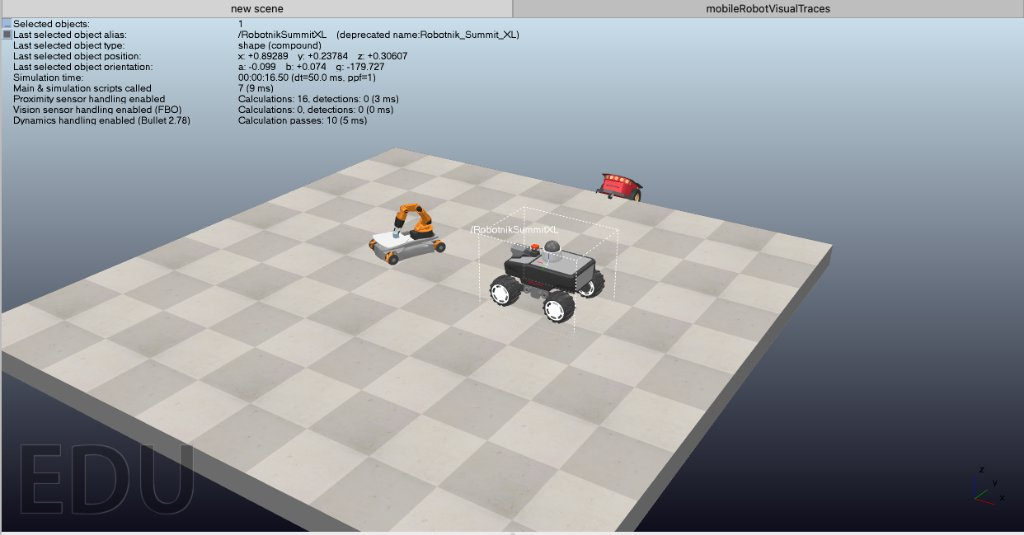
\includegraphics[width=\linewidth]{fig_task4_simulated.png}
  \end{subfigure}
  \caption{Robot models placed in the scene (left) and dynamic motion during simulation (right).}
  \label{fig:task4_simulation}
\end{figure}

% =============================================================================
% TASK 5: SIMULATOR DEMO SCENES
% =============================================================================
\subsubsection*{Task 5: Demo Scene Execution}
Two pre-built demo scenes were executed:

\paragraph{Demo 1: \texttt{mobileRobotVisualTraces.ttt}}
Mobile robots navigate reactively while generating visual trajectory traces.

\begin{figure}[H]
  \centering
  \begin{subfigure}[b]{0.48\linewidth}
    \centering
    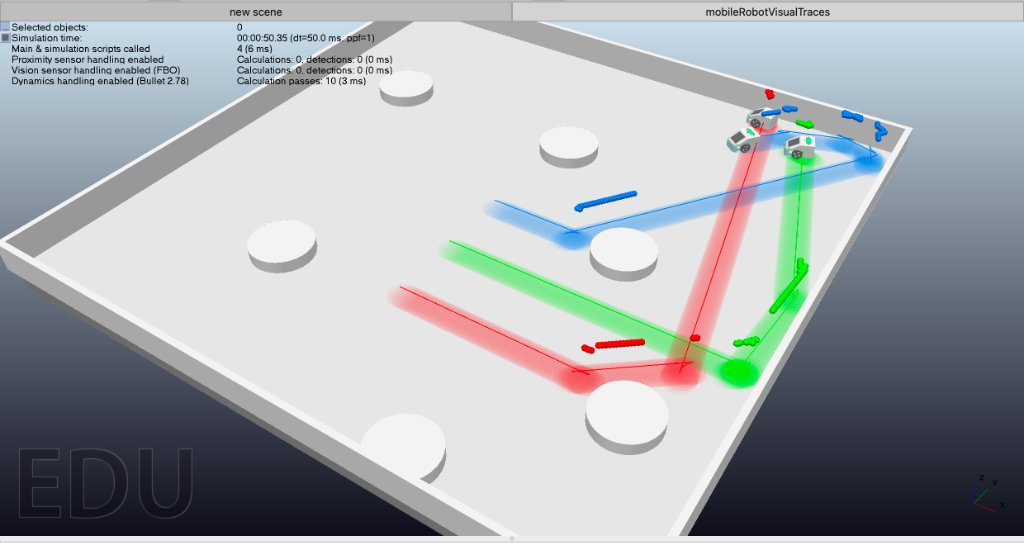
\includegraphics[width=\linewidth]{fig_task5_traces_1.png}
  \end{subfigure}
  \hfill
  \begin{subfigure}[b]{0.48\linewidth}
    \centering
    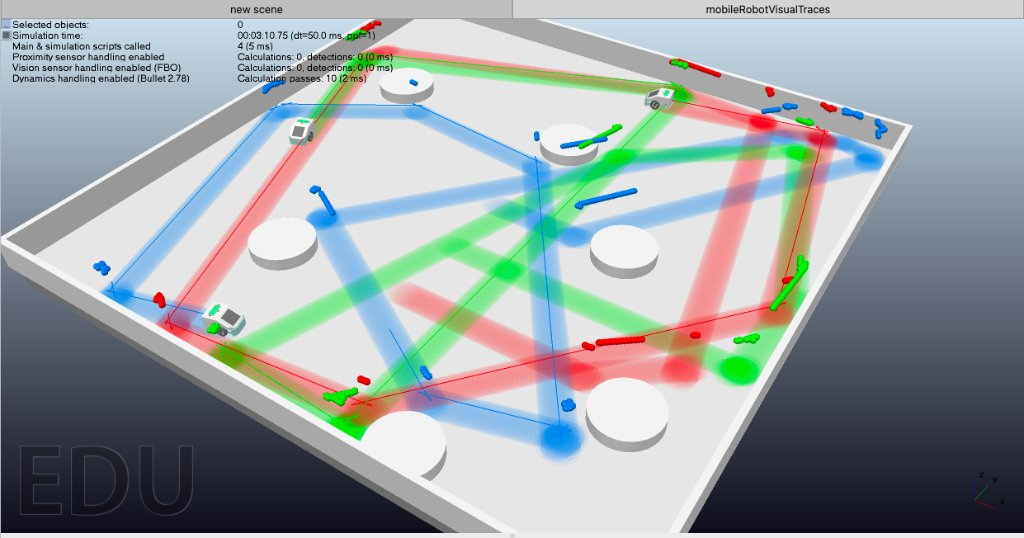
\includegraphics[width=\linewidth]{fig_task5_traces_2.png}
  \end{subfigure}
  \caption{\texttt{mobileRobotVisualTraces} scene at $t=50\,\text{s}$ (left) and $t=3\,\text{min}$ (right).}
  \label{fig:task5_demo_traces}
\end{figure}

\paragraph{Demo 2: \texttt{navigationWithinAPointCloud.ttt}}
A Pioneer P3DX navigates inside a 3D point cloud mesh using proximity sensor rays for obstacle detection.

\begin{figure}[H]
  \centering
  \begin{subfigure}[b]{0.48\linewidth}
    \centering
    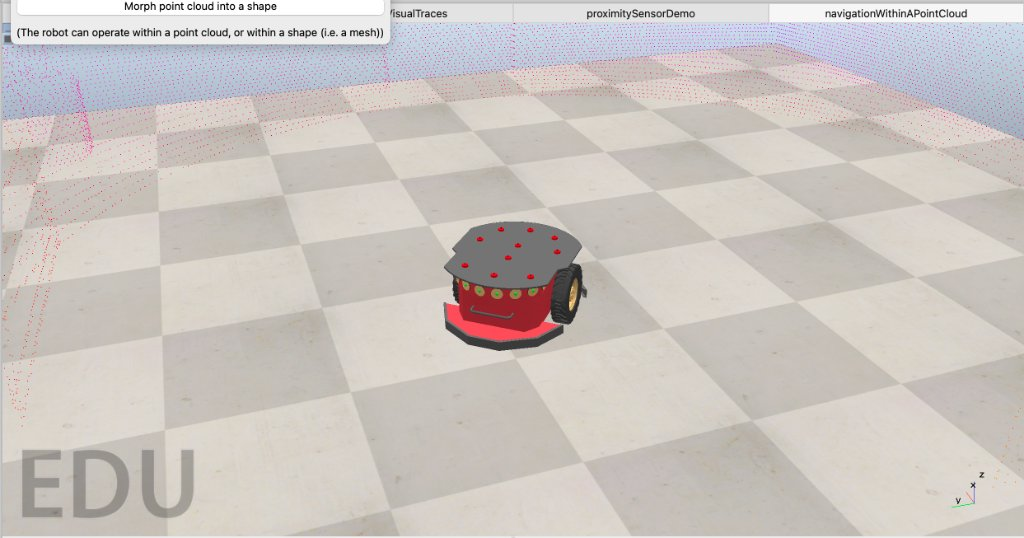
\includegraphics[width=\linewidth]{fig_task5_pointcloud_1.png}
  \end{subfigure}
  \hfill
  \begin{subfigure}[b]{0.48\linewidth}
    \centering
    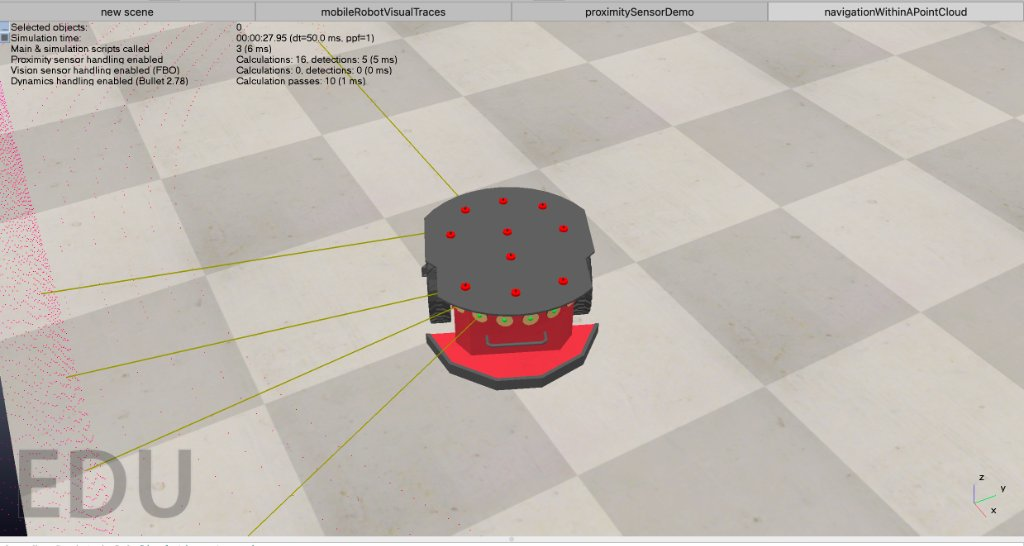
\includegraphics[width=\linewidth]{fig_task5_pointcloud_2.png}
  \end{subfigure}
  \caption{\texttt{navigationWithinAPointCloud} initial scene (left) and active sensor ray-casting (right).}
  \label{fig:task5_demo_pointcloud}
\end{figure}

% =============================================================================
% TASK 6: COPPELIASIM TUTORIAL (BUBBLEROB)
% =============================================================================
\subsubsection*{Task 6: Simulator Tutorial Execution (BubbleRob)}
The official \texttt{BubbleRob} tutorial was executed to study differential-drive robot modeling. It demonstrates two actuated wheels, a passive caster, proximity sensor ray-casting for obstacle avoidance, vision sensor processing, and real-time distance plotting.

\begin{figure}[H]
  \centering
  \begin{subfigure}[b]{0.48\linewidth}
    \centering
    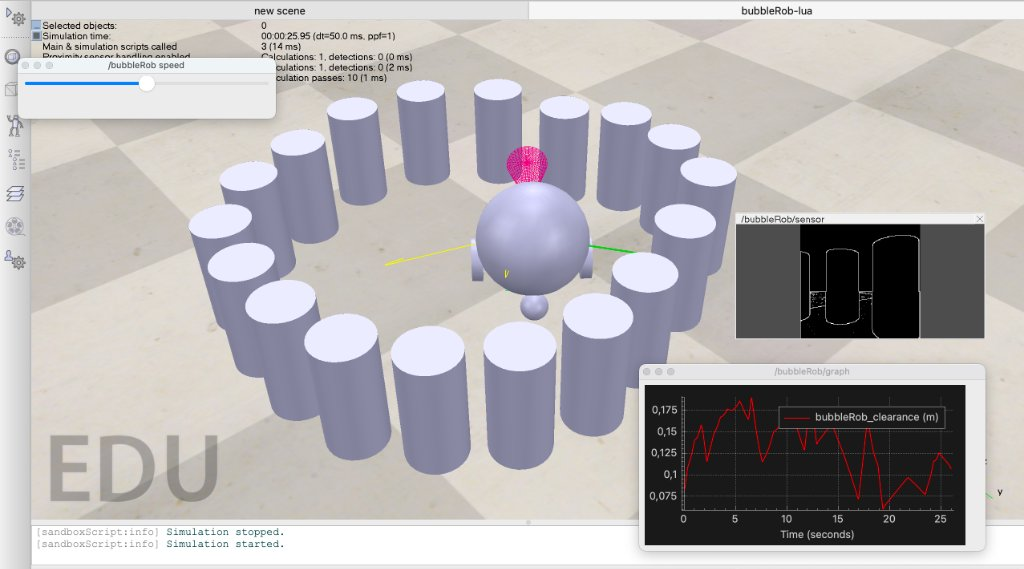
\includegraphics[width=\linewidth,height=3.8cm,keepaspectratio]{fig_task6_bubblerob_1.png}
  \end{subfigure}
  \hfill
  \begin{subfigure}[b]{0.48\linewidth}
    \centering
    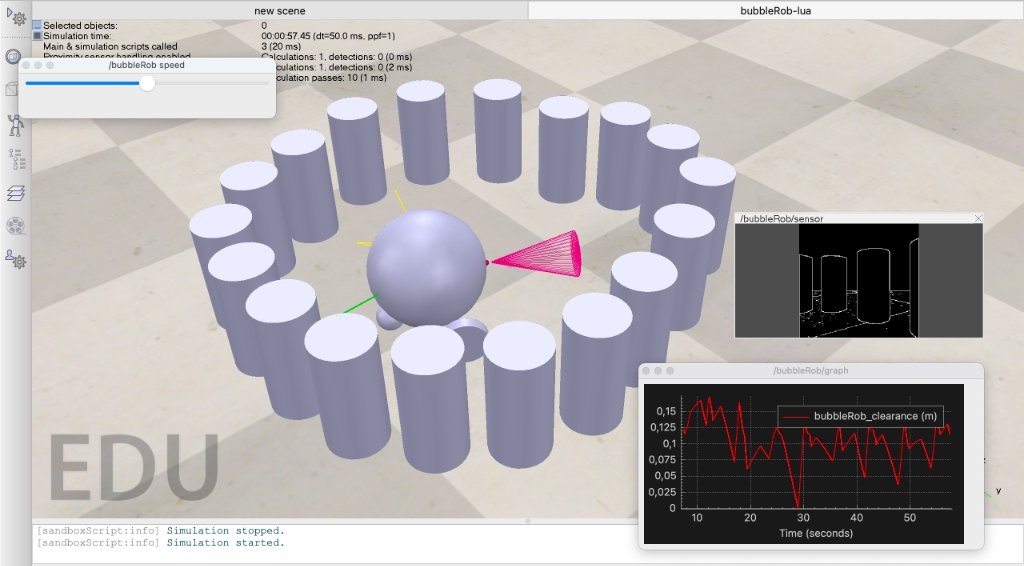
\includegraphics[width=\linewidth,height=3.8cm,keepaspectratio]{fig_task6_bubblerob_2.png}
  \end{subfigure}
  \caption{\texttt{BubbleRob} tutorial simulation showing proximity cone ray-casting, vision sensing, and clearance graph.}
  \label{fig:task6_bubblerob}
\end{figure}

% =============================================================================
% SECTION 1.4: ROS 2 INTERFACE INSTALLATION AND TESTING
% =============================================================================
\subsection*{1.4 ROS 2 Interface}

\subsubsection*{1.4.1 Installation and Compilation}
The \texttt{sim\_ros2\_interface} package was configured with the lab's \texttt{interfaces.txt} and compiled using \texttt{colcon build}:

\begin{figure}[H]
  \centering
  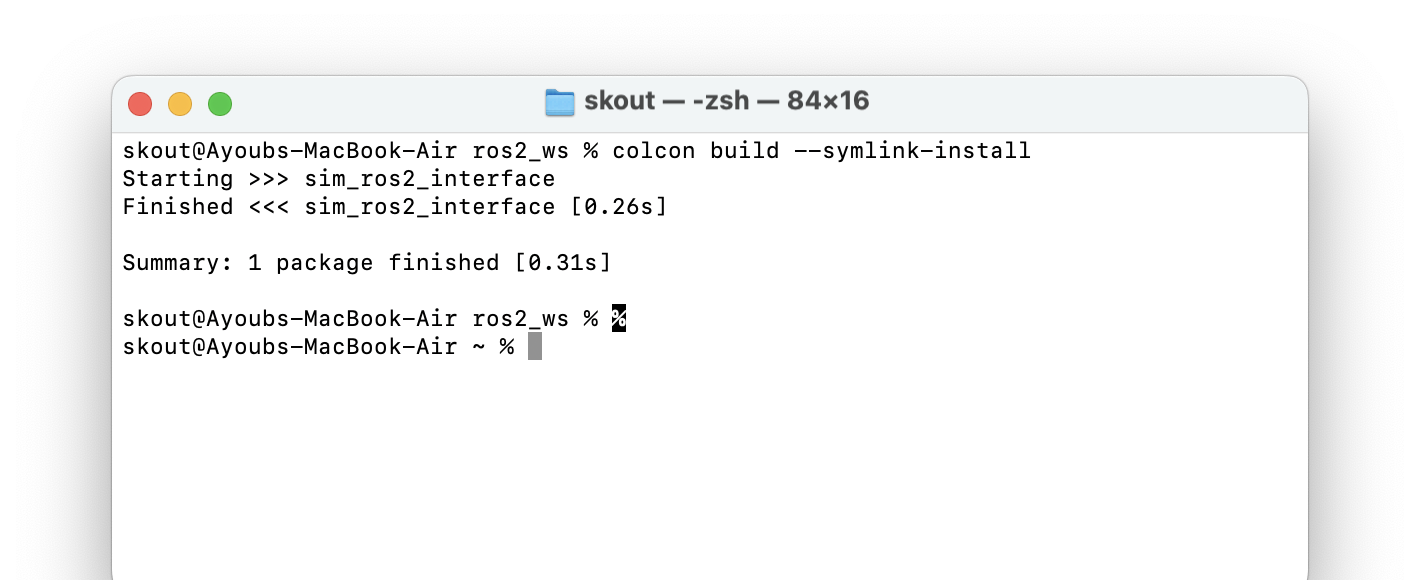
\includegraphics[width=0.86\linewidth,height=3.2cm,keepaspectratio]{fig_1_4_colcon_build.png}
  \caption{Successful compilation and installation of \texttt{sim\_ros2\_interface} via \texttt{colcon build}.}
  \label{fig:colcon_build}
\end{figure}

\subsubsection*{1.4.2 Testing the ROS 2 Interface}
With CoppeliaSim running the \texttt{ENSIA\_IMR\_Lab2.ttt} scene, active nodes and simulation topics were verified:

\begin{figure}[H]
  \centering
  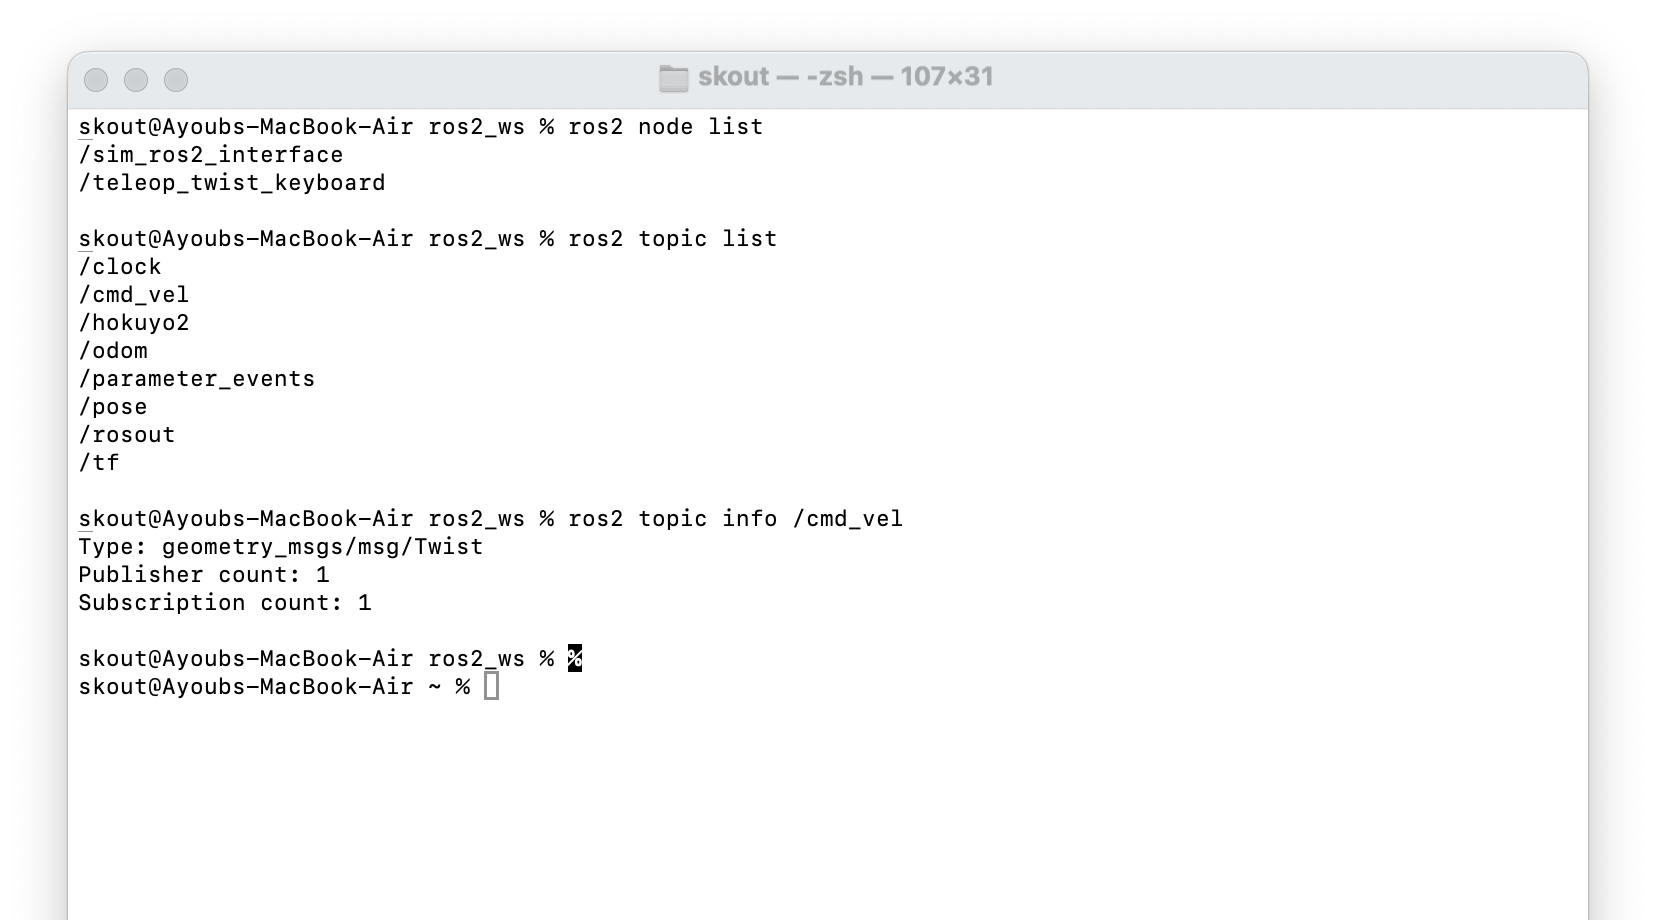
\includegraphics[width=0.86\linewidth,height=3.6cm,keepaspectratio]{fig_1_4_ros2_test.png}
  \caption{Active ROS 2 graph showing the \texttt{/sim\_ros2\_interface} node and registered simulation topics.}
  \label{fig:ros2_nodes_topics}
\end{figure}

\newpage
% =============================================================================
% SECTION 2: DIFFERENTIAL DRIVE ROBOT MOTION MODELING
% =============================================================================
\section{Differential Drive Robot Motion Modeling}
\subsection*{2.2 Tasks}

\subsubsection*{Task 1: Scene Initialization (\texttt{ENSIA\_IMR\_Lab2.ttt})}
The laboratory scene \texttt{ENSIA\_IMR\_Lab2.ttt} was opened in CoppeliaSim, initializing the Pioneer P3DX differential-drive mobile robot, actuated wheel joints, sensors, and the planar ground arena.

\subsubsection*{Task 2: Wheel Angular Velocity Derivation \& Implementation}
From the lab manual, the kinematic relationship of a differential-drive robot is defined by Equations (1) to (4):
\begin{align}
  v &= \frac{v_R + v_L}{2} \label{eq:1} \\
  \omega &= \frac{v_R - v_L}{l} \label{eq:2} \\
  v_R &= r \cdot \dot{\phi}_R \label{eq:3} \\
  v_L &= r \cdot \dot{\phi}_L \label{eq:4}
\end{align}
where $r$ is the wheel radius and $l$ is the wheelbase.

\paragraph{Derivation of $\dot{\phi}_R$ and $\dot{\phi}_L$ from Equations (1) to (4):}
From Equations \eqref{eq:1} and \eqref{eq:2}:
\begin{align*}
  v_R + v_L &= 2v \\
  v_R - v_L &= \omega \cdot l
\end{align*}
Adding the two equations:
\[
  2v_R = 2v + \omega \cdot l \implies v_R = v + \frac{\omega \cdot l}{2}
\]
Subtracting the two equations:
\[
  2v_L = 2v - \omega \cdot l \implies v_L = v - \frac{\omega \cdot l}{2}
\]
Substituting Equations \eqref{eq:3} and \eqref{eq:4} ($v_R = r \cdot \dot{\phi}_R$ and $v_L = r \cdot \dot{\phi}_L$) into the expressions:
\begin{align}
  \dot{\phi}_R &= \frac{2v + \omega \cdot l}{2r} = \frac{v}{r} + \frac{\omega \cdot l}{2r} \label{eq:phi_R} \\[4pt]
  \dot{\phi}_L &= \frac{2v - \omega \cdot l}{2r} = \frac{v}{r} - \frac{\omega \cdot l}{2r} \label{eq:phi_L}
\end{align}
Equations \eqref{eq:phi_R} and \eqref{eq:phi_L} compute the target angular velocities for the right and left wheel joints from incoming \texttt{/cmd\_vel} commands.

\paragraph{Implementation in Pioneer P3DX Lua Script:}
The derived equations were implemented in the \texttt{setVelocity\_cb} callback of the Pioneer P3DX simulation script:

\begin{figure}[H]
  \centering
  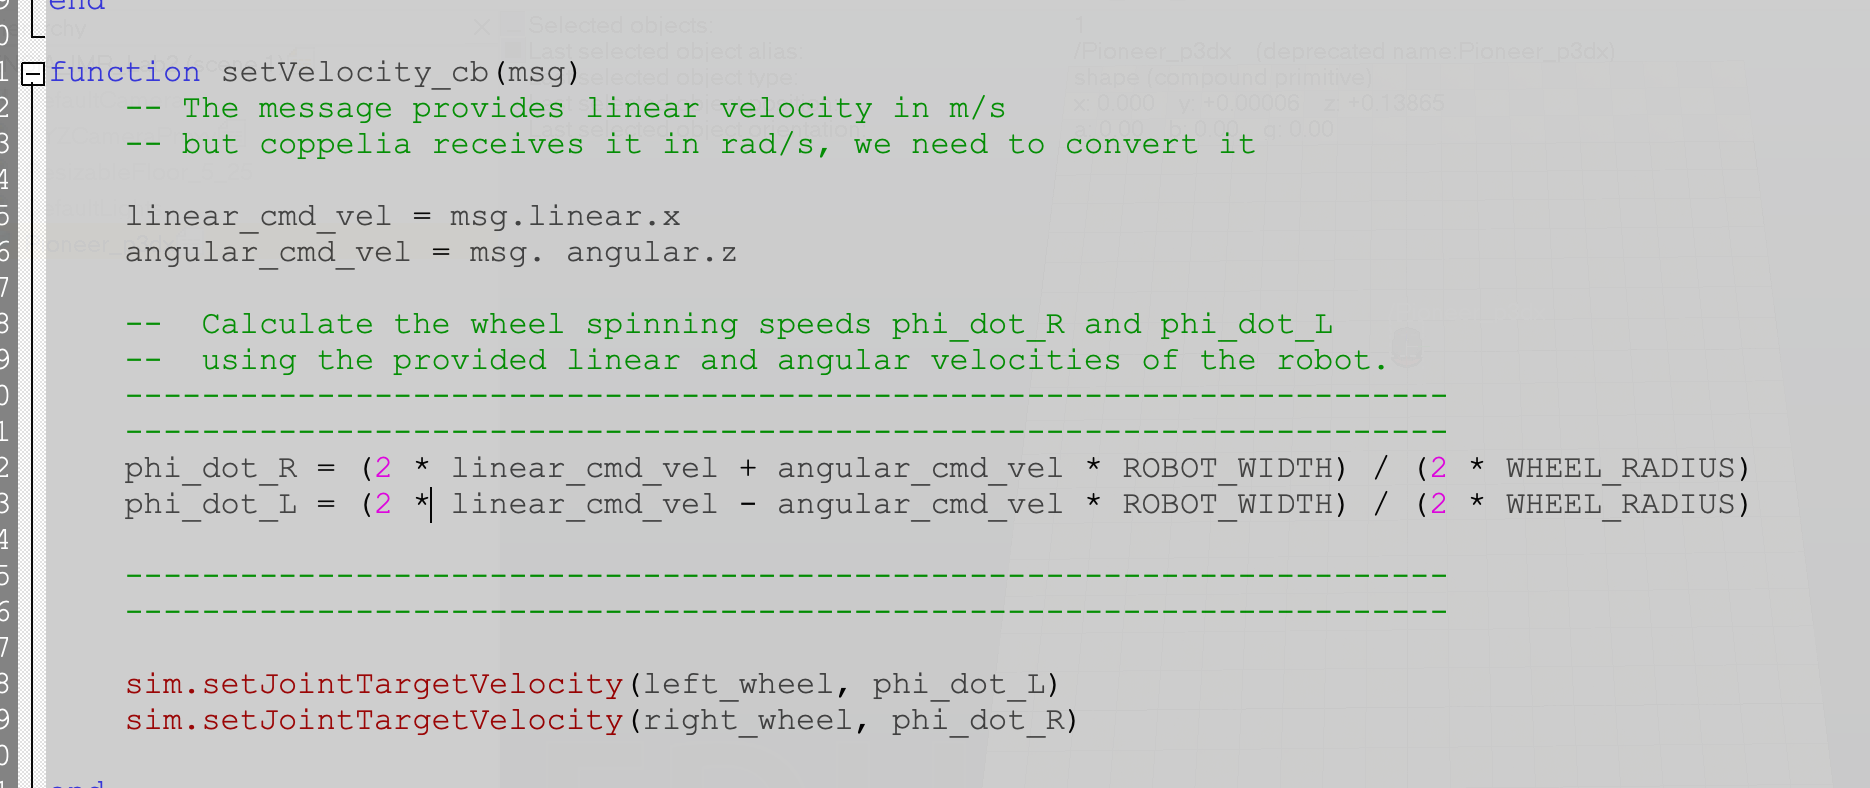
\includegraphics[width=0.88\linewidth]{fig_2_2_lua_script.png}
  \caption{Pioneer P3DX Lua script with the implemented wheel speed calculations in \texttt{setVelocity\_cb}.}
  \label{fig:pioneer_lua_script}
\end{figure}

\subsubsection*{Task 3: Velocity Publishing via ROS 2 CLI}
To verify the kinematic motion model in simulation, the scene was started in CoppeliaSim, and linear and angular velocity commands were published to the \texttt{/cmd\_vel} topic at a frequency of 1\,Hz using the ROS 2 command-line interface:
\begin{lstlisting}[language=bash]
$ ros2 topic pub --rate 1 /cmd_vel geometry_msgs/msg/Twist \
  "{linear: {x: 1.0, y: 0.0, z: 0.0}, angular: {x: 0.0, y: 0.0, z: 1.8}}"
\end{lstlisting}

\paragraph{Kinematic Motion Analysis:}
For the commanded velocities $v = 1.0\,\text{m/s}$ and $\omega = 1.8\,\text{rad/s}$, with Pioneer P3DX parameters $r = 0.0975\,\text{m}$ (wheel radius) and $l = 0.33\,\text{m}$ (wheelbase):
\begin{align*}
  \dot{\phi}_R &= \frac{1.0}{0.0975} + \frac{1.8 \cdot 0.33}{2 \cdot 0.0975} \approx 10.256 + 3.046 = 13.302\,\text{rad/s} \\
  \dot{\phi}_L &= \frac{1.0}{0.0975} - \frac{1.8 \cdot 0.33}{2 \cdot 0.0975} \approx 10.256 - 3.046 = 7.210\,\text{rad/s}
\end{align*}
Because $\dot{\phi}_R > \dot{\phi}_L$, the right wheel spins faster than the left wheel, resulting in a counter-clockwise circular trajectory with turning radius $R = v / \omega = 1.0 / 1.8 \approx 0.556\,\text{m}$.

\begin{figure}[H]
  \centering
  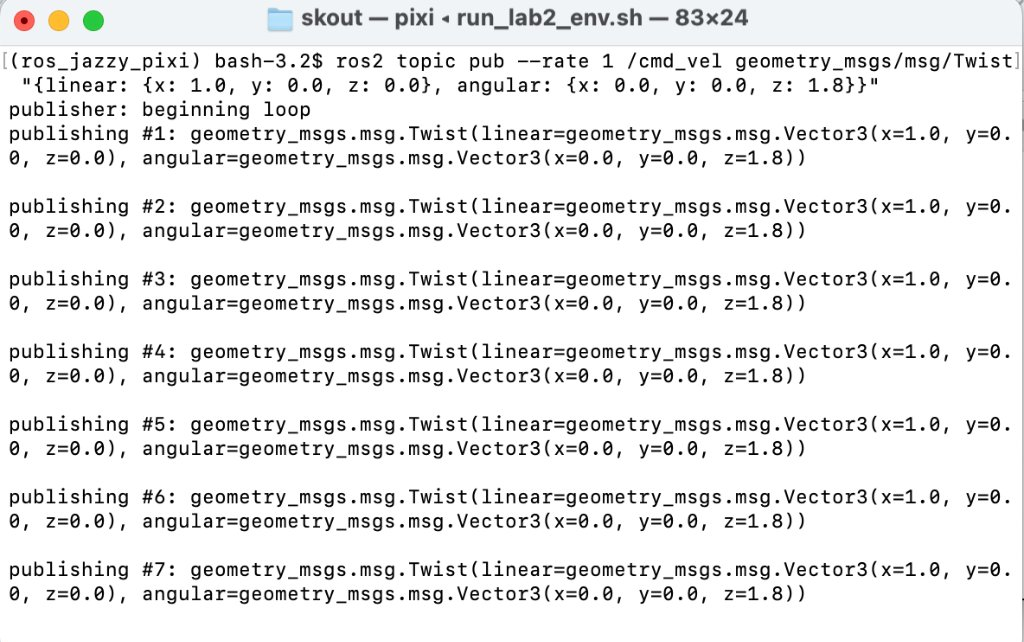
\includegraphics[width=0.85\linewidth,height=5.5cm,keepaspectratio]{fig_2_3_cmdvel_terminal.png}
  \caption{Publishing continuous Twist velocity commands ($v=1.0\,\text{m/s}, \omega=1.8\,\text{rad/s}$) to \texttt{/cmd\_vel} at 1\,Hz.}
  \label{fig:cmdvel_pub}
\end{figure}

\begin{figure}[H]
  \centering
  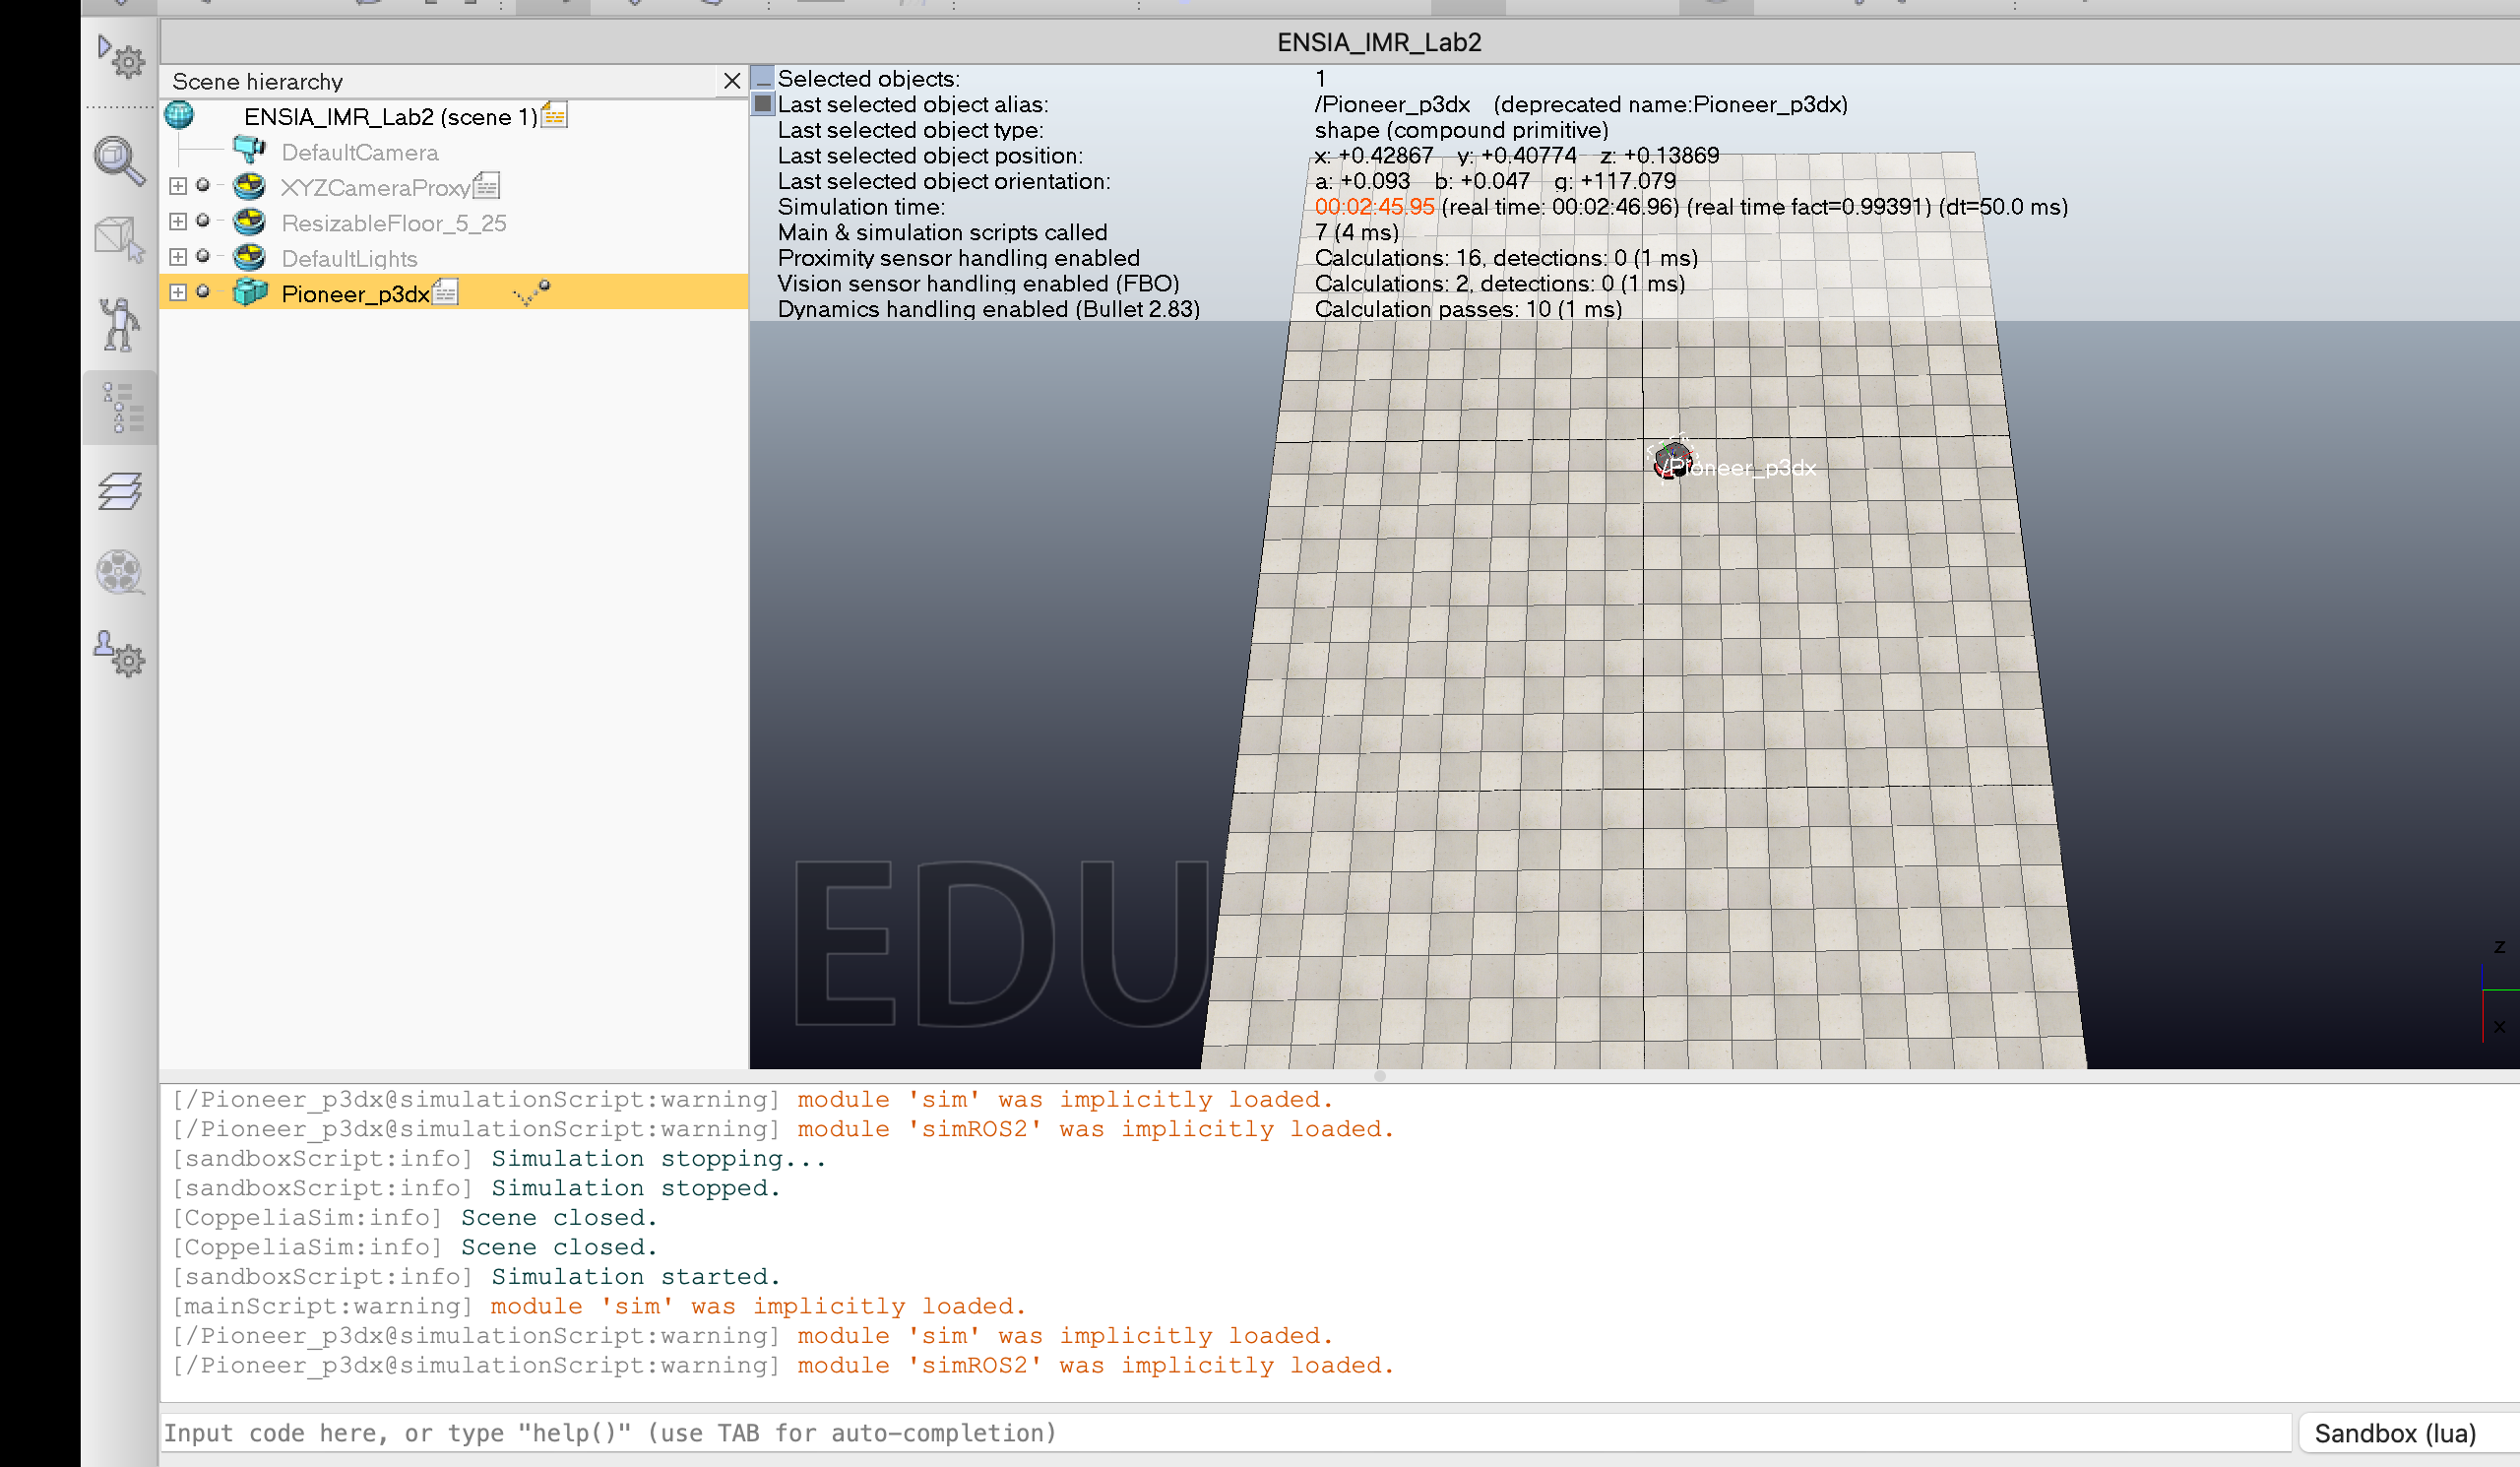
\includegraphics[width=0.96\linewidth,height=10.0cm,keepaspectratio]{fig_2_3_robot_moving_clean.png}
  \caption{Pioneer P3DX executing the circular trajectory in CoppeliaSim corresponding to the received Twist velocities.}
  \label{fig:robot_moving}
\end{figure}

\newpage
\subsubsection*{Task 4: Keyboard Teleoperation Verification}
The \texttt{teleop\_twist\_keyboard} node was executed in the terminal to interactively drive and steer the Pioneer P3DX robot in real time:
\begin{lstlisting}[language=bash]
$ ros2 run teleop_twist_keyboard teleop_twist_keyboard
\end{lstlisting}
Keystrokes were captured by the node and published directly to \texttt{/cmd\_vel}, validating manual teleoperation and dynamic motion in the simulated environment.

\begin{figure}[H]
  \centering
  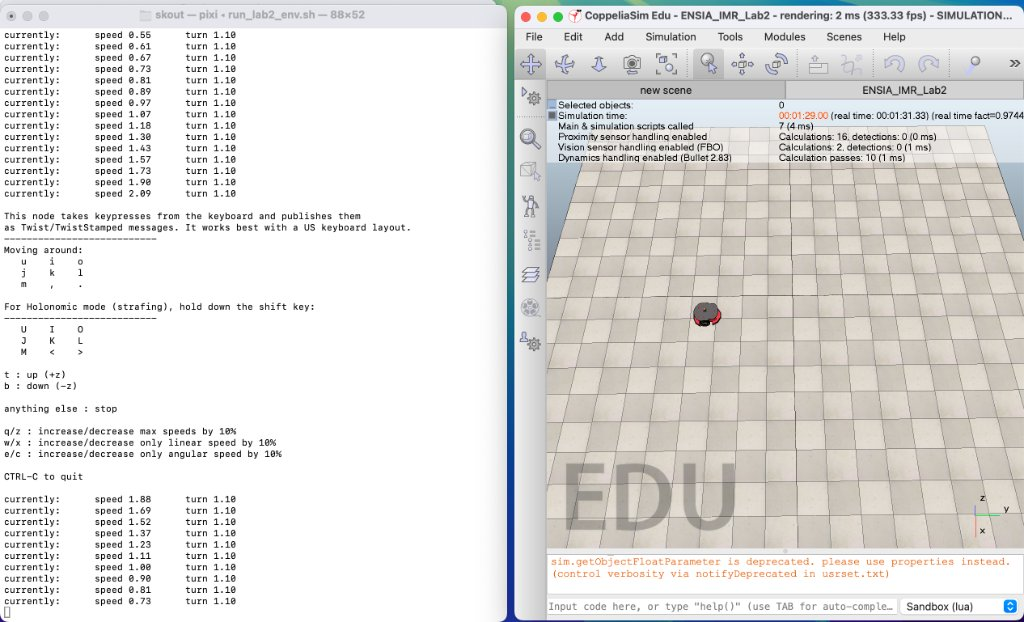
\includegraphics[width=0.95\linewidth,height=7.8cm,keepaspectratio]{fig_2_4_teleop_start.jpg}
  \caption{Initial teleoperation setup: terminal running \texttt{teleop\_twist\_keyboard} side-by-side with CoppeliaSim ($t = 01:29$).}
  \label{fig:teleop_start}
\end{figure}

\begin{figure}[H]
  \centering
  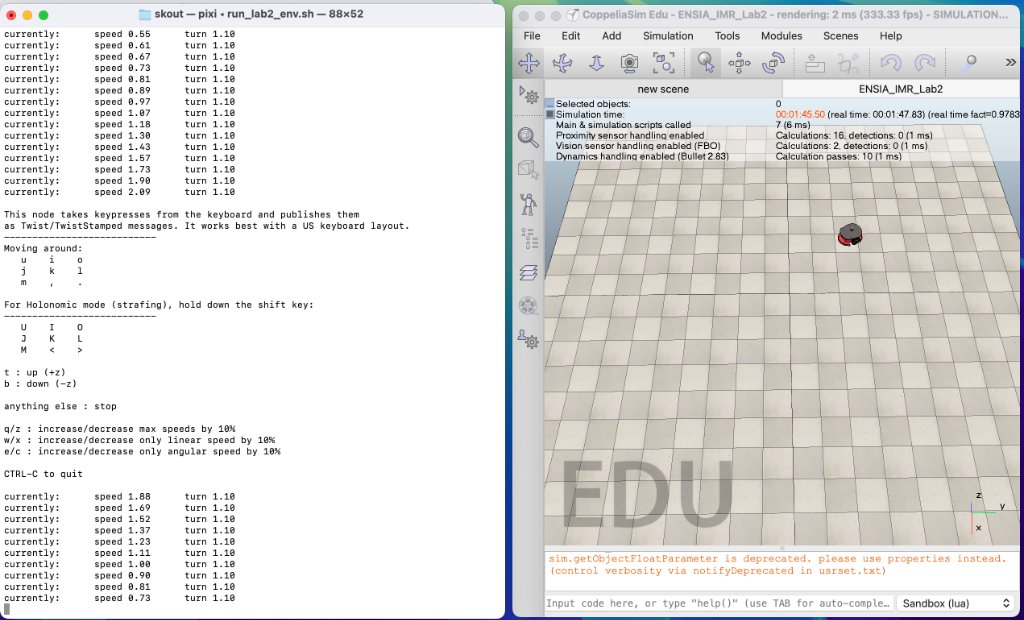
\includegraphics[width=0.95\linewidth,height=7.8cm,keepaspectratio]{fig_2_4_teleop_moved.jpg}
  \caption{Manual trajectory execution: Pioneer P3DX driven forward and steered across the arena floor ($t = 01:45$).}
  \label{fig:teleop_moved}
\end{figure}

\newpage
\subsubsection*{Task 5: Odometry Kinematic Model Implementation in Lua}
The discrete-time forward kinematic model (Equation 5 from the lab manual) was implemented in the Pioneer P3DX Lua script under \texttt{getRobotOdometry()} to compute dead-reckoning pose estimates from wheel encoder speeds:
\begin{align}
  x_{t+\Delta t} &= x_t + v \cos\theta_t \cdot \Delta t \label{eq:odom_x} \\
  y_{t+\Delta t} &= y_t + v \sin\theta_t \cdot \Delta t \label{eq:odom_y} \\
  \theta_{t+\Delta t} &= \theta_t + \omega \cdot \Delta t \label{eq:odom_theta}
\end{align}
where $v = \frac{v_R + v_L}{2}$, $\omega = \frac{v_R - v_L}{l}$, and $\Delta t = \texttt{sim.getSimulationTimeStep()}$.

\begin{figure}[H]
  \centering
  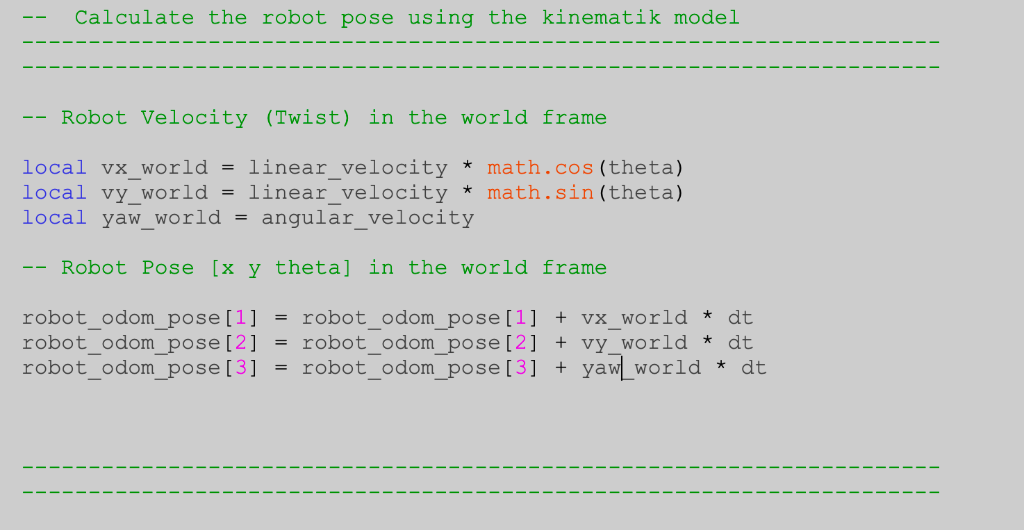
\includegraphics[width=0.92\linewidth,height=4.6cm,keepaspectratio]{fig_2_5_odom_lua.png}
  \caption{Implemented odometric pose integration in the Pioneer P3DX Lua script (\texttt{getRobotOdometry}).}
  \label{fig:odom_lua}
\end{figure}

\subsubsection*{Task 6: Odometry vs. Ground Truth Pose Verification via Topic Echo}
To verify the implemented odometry model against ground truth, the simulation was started, the Pioneer was teleoperated using \texttt{teleop\_twist\_keyboard}, and both topics were echoed simultaneously in separate terminals:
\begin{lstlisting}[language=bash]
$ ros2 topic echo /odom    # Calculated odometric pose (with encoder noise)
$ ros2 topic echo /pose    # Ground truth pose from CoppeliaSim
\end{lstlisting}

\begin{figure}[H]
  \centering
  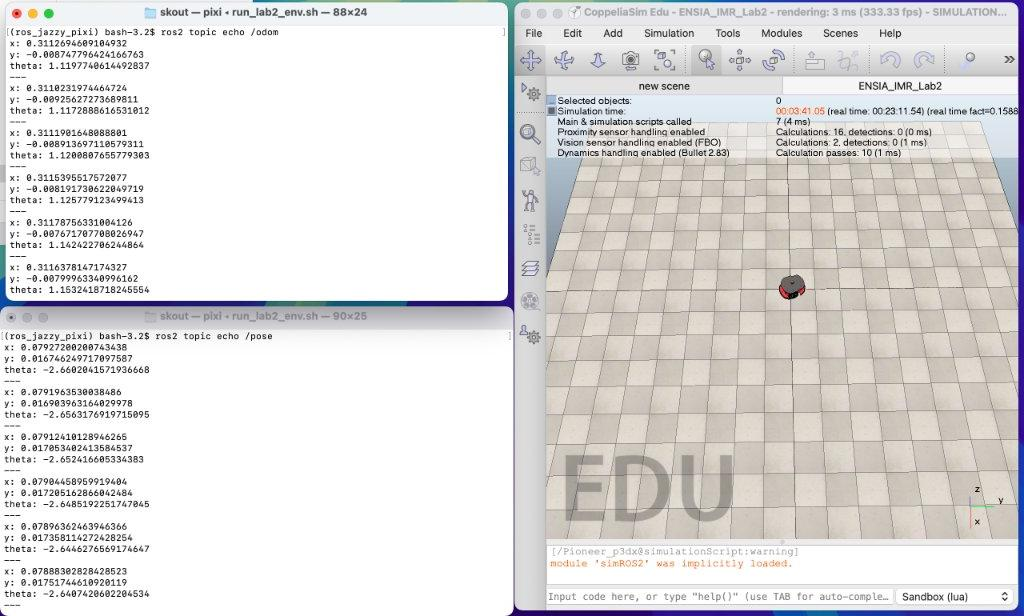
\includegraphics[width=0.95\linewidth,height=7.8cm,keepaspectratio]{fig_2_6_odom_pose_echo.jpg}
  \caption{Simultaneous topic echo: calculated noisy odometry (\texttt{/odom}, top) versus ground truth (\texttt{/pose}, bottom) during robot motion in CoppeliaSim.}
  \label{fig:odom_pose_echo}
\end{figure}

\newpage
\subsubsection*{Task 7: ROS 2 Bag Recording, Inspection, and Playback}
All active ROS 2 topics published during the robot simulation and teleoperation were recorded into a standard ROS 2 bag file using \texttt{ros2 bag record}:
\begin{lstlisting}[language=bash]
$ cd ~/ENSIA/Y4/S7/ROBOTICS/LABS/2
$ ros2 bag record -a -o Lab2_BELHIMER_Mohamed_Ayoub
\end{lstlisting}

\begin{figure}[H]
  \centering
  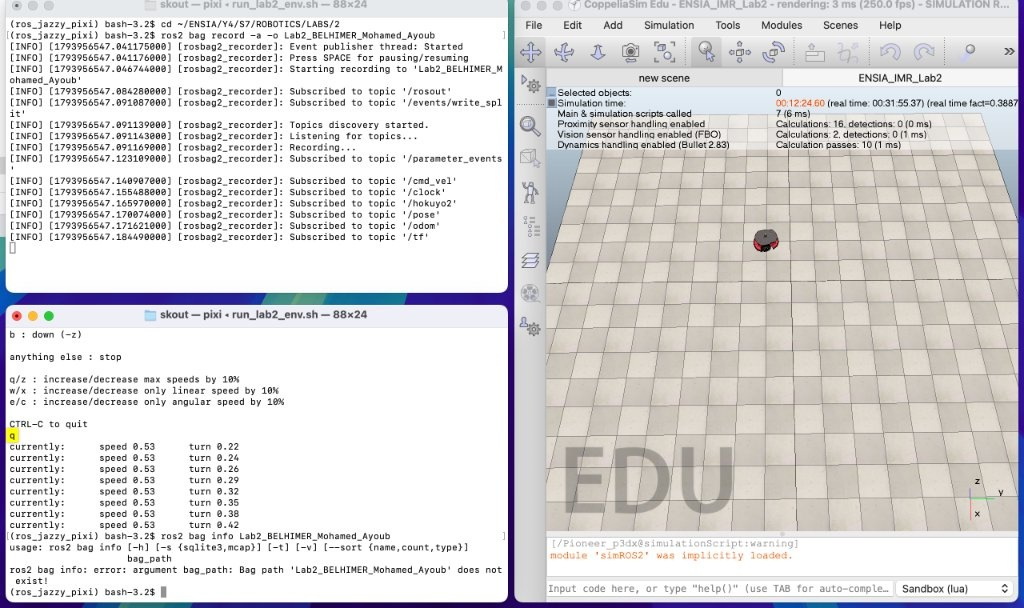
\includegraphics[width=0.95\linewidth,height=5.2cm,keepaspectratio]{fig_2_7_bag_record.jpg}
  \caption{Simultaneous topic recording using \texttt{ros2 bag record -a} while teleoperating the Pioneer P3DX in CoppeliaSim.}
  \label{fig:bag_record}
\end{figure}

The recorded bag structure and topic metadata were verified via \texttt{ros2 bag info}:
\begin{lstlisting}[language=bash,basicstyle=\ttfamily\scriptsize]
$ ros2 bag info Lab2_BELHIMER_Mohamed_Ayoub

Files:             Lab2_BELHIMER_Mohamed_Ayoub_0.mcap
Bag size:          4.9 MiB
Storage id:        mcap  |  ROS Distro: jazzy
Duration:          80.389s  |  Messages: 7773
Topic information:
  /clock      | Count: 1540 | Type: rosgraph_msgs/msg/Clock
  /cmd_vel    | Count: 56   | Type: geometry_msgs/msg/Twist
  /hokuyo2    | Count: 1541 | Type: sensor_msgs/msg/LaserScan
  /odom       | Count: 1540 | Type: geometry_msgs/msg/Pose2D
  /pose       | Count: 1540 | Type: geometry_msgs/msg/Pose2D
  /tf         | Count: 1541 | Type: tf2_msgs/msg/TFMessage
  /rosout     | Count: 15   | Type: rcl_interfaces/msg/Log
\end{lstlisting}

To replay the recorded mission for offline evaluation, topic monitoring, or visualization, the bag is replayed using \texttt{ros2 bag play}:
\begin{lstlisting}[language=bash]
$ cd ~/ENSIA/Y4/S7/ROBOTICS/LABS/2
$ ros2 bag play Lab2_BELHIMER_Mohamed_Ayoub --loop
\end{lstlisting}

\begin{figure}[H]
  \centering
  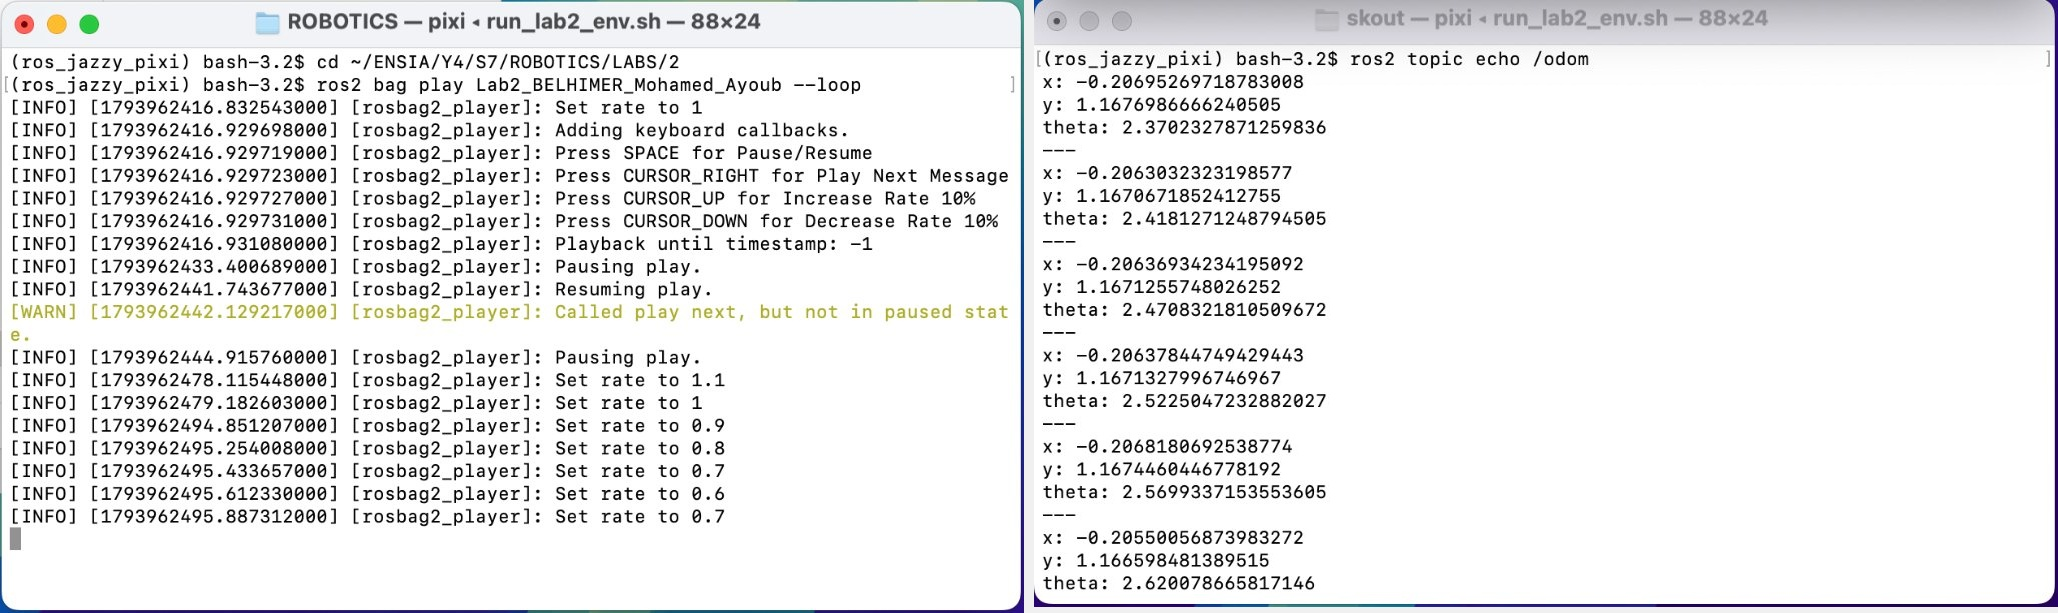
\includegraphics[width=0.98\linewidth,height=4.5cm,keepaspectratio]{fig_2_7_bag_playback_combined.jpg}
  \caption{Offline mission playback verification: interactive playback execution with rate adjustment (left) alongside live topic subscription via \texttt{ros2 topic echo /odom} (right).}
  \label{fig:bag_playback}
\end{figure}

\newpage
\subsubsection*{Task 8: PlotJuggler Trajectory and Pose Visualization}
PlotJuggler was launched via ROS 2 to visualize and analyze the temporal and spatial evolution of the robot state recorded in \texttt{Lab2\_BELHIMER\_Mohamed\_Ayoub}:
\begin{lstlisting}[language=bash]
$ ros2 run plotjuggler plotjuggler
\end{lstlisting}

\begin{figure}[H]
  \centering
  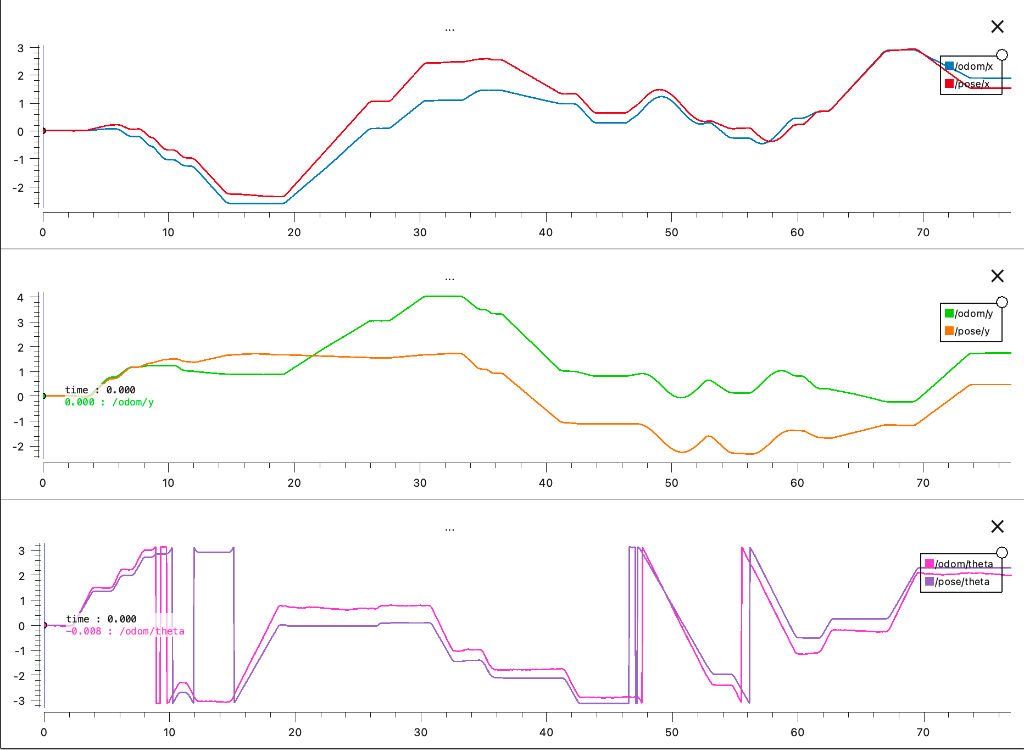
\includegraphics[width=0.95\linewidth,height=8.0cm,keepaspectratio]{fig_2_8_plotjuggler_timeseries.png}
  \caption{PlotJuggler temporal tracking: comparing calculated odometry (\texttt{/odom}) against ground truth (\texttt{/pose}) for $x(t)$ (top), $y(t)$ (middle), and $\theta(t)$ (bottom) over the 80-second mission.}
  \label{fig:plotjuggler_timeseries}
\end{figure}

\begin{figure}[H]
  \centering
  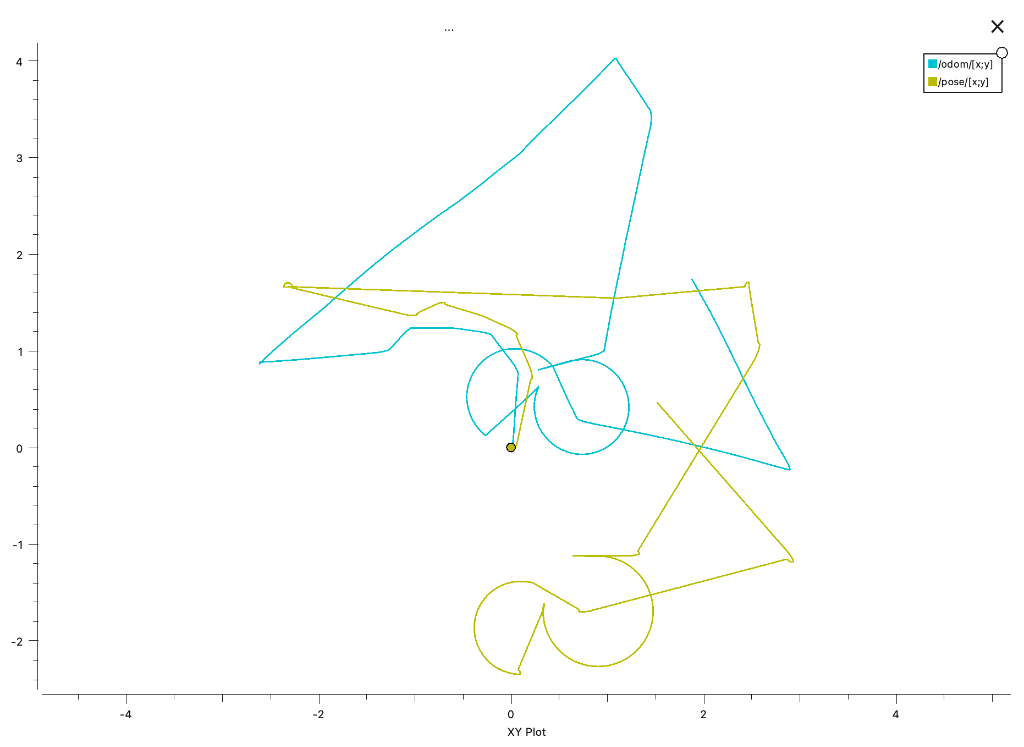
\includegraphics[width=0.92\linewidth,height=7.5cm,keepaspectratio]{fig_2_8_plotjuggler_xypath.png}
  \caption{PlotJuggler 2D Cartesian path ($y$ vs. $x$): calculated odometric path (\texttt{/odom}, cyan) versus actual ground truth path (\texttt{/pose}, yellow-green) starting at $(0, 0)$.}
  \label{fig:plotjuggler_xypath}
\end{figure}

\newpage
\subsubsection*{Task 9: Final Pose Error Computation}
To quantify the accumulated dead-reckoning drift over the recorded teleoperation trajectory, the final pose from the odometry calculation was evaluated against the true simulator pose using the error metrics specified in the lab manual:
\begin{align}
  \text{Position\_Error} &= \sqrt{(x_{\text{true}} - x_{\text{odom}})^2 + (y_{\text{true}} - y_{\text{odom}})^2} \label{eq:pos_err} \\
  \text{Orientation\_Error} &= \sqrt{(\theta_{\text{true}} - \theta_{\text{odom}})^2} \label{eq:ori_err}
\end{align}

Extracting the terminal state at $t = 80.39\,\text{s}$ yields:
\begin{itemize}
  \item \textbf{Ground Truth Final Pose (\texttt{/pose}):}
  \[
    x_{\text{true}} = 1.5209\,\text{m}, \quad y_{\text{true}} = 0.4623\,\text{m}, \quad \theta_{\text{true}} = 2.2948\,\text{rad} \ (131.48^\circ)
  \]
  \item \textbf{Calculated Odometry Final Pose (\texttt{/odom}):}
  \[
    x_{\text{odom}} = 1.8814\,\text{m}, \quad y_{\text{odom}} = 1.7406\,\text{m}, \quad \theta_{\text{odom}} = 1.9979\,\text{rad} \ (114.47^\circ)
  \]
\end{itemize}

Substituting these coordinates into Equations \eqref{eq:pos_err} and \eqref{eq:ori_err}:
\begin{align*}
  \text{Position\_Error} &= \sqrt{(1.5209 - 1.8814)^2 + (0.4623 - 1.7406)^2} \\
  &= \sqrt{(-0.3605)^2 + (-1.2783)^2} = \sqrt{0.1300 + 1.6340} = \mathbf{1.3281\,\text{m}} \\[6pt]
  \text{Orientation\_Error} &= \sqrt{(2.2948 - 1.9979)^2} = |0.2969| = \mathbf{0.2969\,\text{rad}} \ (\mathbf{17.01^\circ})
\end{align*}

\subsubsection*{Task 10: Results Analysis and Conclusion}
\paragraph{Analysis of Results:}
At the beginning of the simulation ($t = 0$), the calculated odometry (\texttt{/odom}) matches the ground truth pose (\texttt{/pose}) at the origin $(0, 0, 0)$. As the robot moves, the odometric trajectory follows the general shape of the robot motion, including the turns and circular loops.

However, as time progresses, the calculated odometry gradually drifts away from the true robot pose, reaching a final position error of $1.33\,\text{m}$ and an orientation error of $17.01^\circ$ after 80 seconds. This drift occurs because:
\begin{itemize}
  \item Gaussian noise added to the wheel encoder readings accumulates with every integration step ($\Delta t = 50\,\text{ms}$).
  \item Any error in the estimated heading $\theta$ misaligns the calculated velocity components ($v\cos\theta, v\sin\theta$), causing position error to grow continuously.
\end{itemize}

\paragraph{Conclusion:}
This experiment demonstrates that open-loop wheel odometry is only reliable for short periods. Because odometry errors accumulate over time without bound, mobile robots cannot rely solely on wheel odometry for localization and require external sensors (such as LiDAR, cameras, or GPS) to periodically correct the accumulated drift.

\end{document}
